\documentclass[10pt,a4paper,openany]{book}  % 10pt, A4, allow chapters on any page

% Normal margins
\usepackage[margin=2.5cm]{geometry}  % Standard margins


% Single spacing
\usepackage{setspace}
\singlespacing

% Avoid vertical stretching to "flush" bottoms — helps prevent big gaps
\raggedbottom

% Other packages
\usepackage[a-1b]{pdfx}
\usepackage{fourier}
\usepackage[utf8]{inputenc}
\usepackage[T1]{fontenc}
\usepackage[ngerman,italian,english]{babel}
\usepackage{graphicx}
\usepackage{xcolor}
\usepackage{hyphenat}
\usepackage{longtable}
\usepackage{array,booktabs}
\usepackage{pdflscape}
\usepackage{caption}
\usepackage[absolute]{textpos}
\usepackage{pifont}
\usepackage{listings}
\usepackage{enumitem}
\usepackage[dvipsnames]{xcolor}
\usepackage{tikz}
\usepackage{float}

\usepackage{pgfplots}
\pgfplotsset{compat=1.17}



% Localize/rename auto-generated list titles
\addto\captionsenglish{\renewcommand{\contentsname}{Table of Contents}}

\definecolor{codebackground}{RGB}{248, 248, 248}
\definecolor{codecomment}{RGB}{96, 119, 145}
\definecolor{codecommentdark}{RGB}{72, 89, 109}
\definecolor{codestring}{RGB}{194, 84, 70}
\definecolor{codekeyword}{RGB}{3, 130, 172}
\definecolor{codenumber}{RGB}{170, 88, 0}
\definecolor{codeidentifier}{RGB}{0, 0, 0}
\definecolor{codegray}{rgb}{0.5,0.5,0.5}
\definecolor{codepurple}{rgb}{0.58,0,0.82}
\definecolor{backcolour}{rgb}{0.95,0.95,0.92}
\definecolor{cover}{HTML}{647D91}



\hypersetup{hidelinks}

\def\tableheader{continued from previous page.}
\def\tablefooter{Continues on next page.}

% Define a modern style for listings
\lstdefinestyle{mystyle}{
    backgroundcolor=\color{codebackground}, % Subtle gray background
    basicstyle=\ttfamily\footnotesize\color{codeidentifier}, % Modern monospace with color
    commentstyle=\color{codecomment}\itshape, % Blue italic comments
    keywordstyle=\color{codekeyword}\bfseries, % Blue bold keywords
    stringstyle=\color{codestring}, % Red/orange strings
    numberstyle=\tiny\color{codegray}, % Gray line numbers
    breakatwhitespace=false,
    breaklines=true,
    captionpos=b,
    keepspaces=true,
    numbers=left,
    numbersep=8pt,
    showspaces=false,
    showstringspaces=false,
    showtabs=false,
    tabsize=2,
    frame=single, % Add subtle border
    frameround=tttt, % Rounded corners
    rulecolor=\color{codegray!30}, % Light gray border
    xleftmargin=10pt,
    xrightmargin=10pt
}
% Apply the style to all listings
\lstset{style=mystyle}

% Define the TypeScript language without special colors
\lstdefinelanguage{TypeScript}{
  keywords={
    abstract, async, await, boolean, break, case, catch, class, const, continue,
    debugger, default, delete, do, else, enum, export, extends, false, finally,
    for, from, function, get, if, implements, import, in, instanceof, interface,
    let, new, null, of, package, private, protected, public, return, set, static,
    super, switch, this, throw, true, try, type, typeof, var, void, while, with, yield,
    Promise, Map, Set
  },
  keywordstyle=\bfseries,
  ndkeywords={
    Array, Date, eval, hasOwnProperty, Infinity, isFinite, isNaN, isPrototypeOf,
    length, Math, NaN, name, Number, Object, prototype, String, toString, undefined,
    valueOf
  },
  ndkeywordstyle=\bfseries,
  sensitive=false,
  comment=[l]{//},
  morecomment=[s]{/*}{*/},
  morestring=[b]',
  morestring=[b]",
  morestring=[b]`
}

% Custom commands and packages
\lstdefinelanguage{JSON}{
  morestring=[b]",% strings are in double quotes
  morecomment=[l]{//},% comments start with //
  morecomment=[s]{/*}{*/},% comments start with /* and end with */
  morekeywords={true,false,null},% keywords
  sensitive=false,
}

% Set default language for listings
\lstset{language=TypeScript}


% \lstset{language={Java}, aboveskip=3mm,	belowskip=3mm, basicstyle=\ttfamily, keywordstyle=\color{blue}, commentstyle=\color{gray}, stringstyle=\color{orange}, breaklines=true, tabsize=2, numbers=left,	numberstyle=\tiny\color{gray}, numbersep=5pt, prebreak=\mbox{\tiny$\searrow$}, captionpos=b}

% \lstset{
%   literate={\\}{{\textbackslash}}1
%            {_}{{\textunderscore}}1
%            {~}{{\textasciitilde}}1
% }

\renewcommand{\UrlBigBreaks}{\do\:\do\/}
\renewcommand{\UrlBreaks}{\do\/\do\0\do\1\do\2\do\3\do\4\do\5\do\6\do\7\do\8\do\9\do\a\do\b\do\c\do\d\do\e\do\f\do\g\do\h\do\i\do\j\do\k\do\l\do\m\do\n\do\o\do\p\do\q\do\r\do\s\do\t\do\u\do\v\do\w\do\x\do\y\do\z\do\A\do\B\do\C\do\D\do\E\do\F\do\G\do\H\do\I\do\J\do\K\do\L\do\M\do\N\do\O\do\P\do\Q\do\R\do\S\do\T\do\U\do\V\do\W\do\X\do\Y\do\Z}
\mathchardef\UrlBreakPenalty=1000
\mathchardef\UrlBigBreakPenalty=1000

\newenvironment{tight_enumerate}{
\begin{enumerate}
  \setlength{\itemsep}{0pt}  
  \setlength{\parskip}{0pt}
}{\end{enumerate}}

\newenvironment{tight_itemize}{
\begin{itemize}
  \setlength{\itemsep}{0pt}
  \setlength{\parskip}{0pt}
}{\end{itemize}}

\newcommand{\wtf}[1]{{\color{red}#1}}

\newcommand{\scenario}[9]{
{
\setlength{\tabcolsep}{6pt}
\begin{longtable}[l]{>{\raggedright}p{3cm}p{10.5cm}}
\caption{Quality scenario QS#1 for quality requirement #2} 
\\

\hline\noalign{\smallskip}
Aspect & Description \\[2pt]
\hline
\endfirsthead
 
\multicolumn{2}{l}{\tablename\ \thetable{}, \tableheader}\\
\hline\noalign{\smallskip}
Aspect & Description \\[2pt]
\hline
\endhead

\multicolumn{2}{r}{\tablefooter} \\
\endfoot

\noalign{\smallskip}\hline\noalign{\smallskip}
\endlastfoot

No.                & QS#1 \\\hline
Property           & #3 \\\hline
Source of stimulus & #4 \\\hline
Stimulus           & #5 \\\hline
Environment        & #6 \\\hline
Artifact           & #7 \\\hline
Response           & #8 \\\hline
Response measure   & #9 \\

\end{longtable}
}
}

\makeatletter
\def\longtableheader{%
  \multicolumn{\LT@cols}{l}{\tablename\ \thetable{}, \tableheader}\\}
\def\longtablefooter{%
  \bottomrule\multicolumn{\LT@cols}{r}{\tablefooter}\endfoot\bottomrule\endlastfoot}
\makeatother

\newcolumntype{L}[1]{>{\raggedright\let\newline\\\arraybackslash\hspace{0pt}}m{#1}}
\newcolumntype{C}[1]{>{\centering\let\newline\\\arraybackslash\hspace{0pt}}m{#1}}
\newcolumntype{R}[1]{>{\raggedleft\let\newline\\\arraybackslash\hspace{0pt}}m{#1}}

\AtBeginEnvironment{longtable}{\setlength{\tabcolsep}{6pt}}

% Use this only if you have a lot of code
%\AtBeginEnvironment{lstlisting}{\small}

\renewcommand{\lstlistingname}{Listing}
\renewcommand{\lstlistlistingname}{List of Listings}

\def\titleOfTheThesis{Pista: A GenAI-Powered System for Automated Startup Pitch Evaluation}
\def\author{}

\def\candidate{}
\def\supervisor{}
\def\cosupervisor{}
\def\date{2024/2025}
\def\curriculum{Bachelor in Computer Science}
\def\typeOfThesis{Bachelor Thesis}

\begin{document}
\frontmatter
% spell-checker:disable
\begin{titlepage}
  \begin{flushleft}
    
\includegraphics{img/unibz-logo.jpg}
  \end{flushleft}
  
   \begin{flushleft}
    \textcolor{cover}{\normalsize Degree Course}\\[0.5cm]
    \textcolor{cover}{\bfseries \Huge BACHELOR IN INFORMATIK\\
    \Huge CORSO DI LAUREA IN INFORMATICA\\
    \vspace{0.5cm}
    \Huge BACHELOR IN COMPUTER SCIENCE}\\
    \end{flushleft}
    \begin{center}

    \vspace{2.5cm}
    \begin{flushleft}
    \textcolor{cover}{\huge \bfseries \titleOfTheThesis}
  \end{flushleft}
    
   \begin{flushleft}
    \vspace{4.5cm}
      \textcolor{cover}{\large \textbf{Student}}\\
      \textcolor{cover}{\candidate}
      
      \vspace{1cm}
      \textcolor{cover}{ \large \textbf{Berichterstatter / relatore / Supervisor}}\\
      \textcolor{cover}{\supervisor}
      
      \vspace{1cm}
      \textcolor{cover}{\large \textbf{Zweitbetreuer / correlatore / Second Supervisor}}\\
      \textcolor{cover}{\cosupervisor}
      
      \vspace{1cm}
      \textcolor{cover}{\large \textbf{akademisches Jahr / anno accademico / academic Year}}\\
      \textcolor{cover}{\date}
    \end{flushleft}
    
    % Add the university seal at the bottom right
    \vspace{-3.4cm}
    \begin{flushright}
      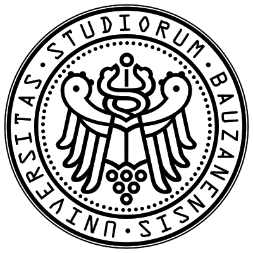
\includegraphics[scale=0.33]{img/university-seal.png}
    \end{flushright}
  \end{center}
\end{titlepage}

% \chapter*{Abstract}
% Startup pitch evaluation has traditionally relied on human expert judgment, which creates inconsistency, scalability challenges, and accessibility barriers. This thesis presents Pista, a GenAI-powered system for automated startup pitch evaluation that addresses these limitations. The system uses GPT-4 to evaluate pitches across four dimensions: Problem-Solution Fit, Business Model \& Market, Team \& Execution, and Pitch Quality. It processes multiple input formats including text submissions and audio recordings.

% The evaluation compares Pista against Winds2Ventures, a commercial startup evaluation platform. Analysis of 22 startup pitches shows 27.3\% alignment within a one-point margin. Pista exhibits systematic optimism with an average 2.0-point positive bias compared to the commercial benchmark. The system demonstrates operational advantages including faster evaluation times (30-60 seconds), lower costs (\$0.10-0.15 per evaluation), and 24/7 availability.

% Dimensional analysis reveals varying performance across evaluation categories. Pista scores highest in Problem-Solution Fit (7.4) and lowest in Team \& Execution (6.7). Sectoral analysis shows technology pitches have the greatest score dispersion, while healthcare pitches achieve highest convergence (50.0\%).

% The implementation uses Next.js 15, React 18, Convex database, and Clerk authentication. The system supports real-time evaluation progress tracking and provides structured feedback with specific improvement recommendations. Performance optimization includes component lazy loading, edge runtime deployment, and comprehensive error handling.

% Current AI evaluation systems need significant calibration before approaching commercial platform reliability. The system faces inherent limitations. It relies on text transcription rather than visual cues, body language, and vocal intonation that human judges use. However, the results demonstrate AI's potential for scalable startup pitch screening. The system's consistency and accessibility advantages make it valuable for initial evaluation stages. This particularly benefits entrepreneurs in underrepresented regions with limited access to expert networks.

% Future enhancements could address current limitations. Interactive pitch sessions with real-time multimodal analysis would improve evaluation depth. AI-generated follow-up questions using video technology could simulate investor interactions. These developments would bridge the gap between current text-based evaluation and comprehensive human judgment. They would maintain operational advantages. 

%This is only needed for a bachelor thesis
% % spell-checker:disable
\begin{otherlanguage}{italian}
\chapter*{Riassunto}

% \begin{description}
%   \item[Motivazione] 

%   \item[Problema] 

%   \item[Approccio] 

%   \item[Risultati] 

%   \item[Conclusioni]
% \end{description}
\end{otherlanguage} 
% % spell-checker:disable
\begin{otherlanguage}{ngerman}
\chapter*{Zusammenfassung}

% \begin{description}
%   \item[Motivation] 

%   \item[Problemstellung] 

%   \item[Ansatz] 

%   \item[Ergebnisse] 

%   \item[Fazit]
% \end{description}
\end{otherlanguage} 

% \chapter*{Acknowledgements}
\label{ch:acknowledgements}

I would like to express my sincere gratitude to everyone who made this thesis possible.

First and foremost, I thank my thesis supervisor for their exceptional guidance, support, and valuable feedback throughout this research project. Their expertise in entrepreneurship and technology was instrumental in shaping both the technical implementation of Pista and the research methodology. I am particularly grateful for their facilitation of the comparative analysis with Winds2Ventures, which enabled the statistical validation that forms the core of this thesis. Their mentorship helped me navigate the complexities of GenAI evaluation systems and statistical analysis.

I extend my appreciation to the Winds2Ventures team for generously providing access to their evaluation platform for comparative research. Their willingness to participate in this academic study contributed significantly to the depth and validity of the analysis. This collaboration exemplifies the value of industry-academia partnerships in advancing research.

I thank the university entrepreneurship programs and competition organizers who provided access to the startup pitch datasets used in this research. Their openness to share these materials enabled the empirical validation of both evaluation systems and made the statistical comparison possible.

Special thanks to the open-source community and the developers of Next.js, Convex, OpenAI, and other technologies that made building Pista possible. Their tools and documentation enabled rapid development and deployment of a full-featured evaluation platform.

I am grateful to my professors and classmates who provided feedback during presentations and discussions that helped refine my understanding of the research questions and methodology.

Finally, I thank my family and friends for their unwavering patience, understanding, and encouragement during the research and writing process. Their support kept me motivated through challenging moments and helped maintain perspective on the broader goals of this work.

This research was conducted with integrity and academic honesty. Any remaining limitations, errors, or omissions are entirely my responsibility.


\tableofcontents
\listoftables
\listoffigures
\lstlistoflistings

\mainmatter

\chapter{Introduction}

\label{ch:introduction}

Getting feedback on startup ideas is crucial for success. Startup founders need to pitch their ideas to investors and get useful feedback to improve their businesses. Research shows that investment decisions depend heavily on the quality of pitch presentations, which play a major role in securing financial support\cite{masterpresentat}. Many business functions have been changed substantially through technology improvements. However, pitch evaluation has not evolved much and still relies on in-person presentations and individual expert judgment.

This thesis investigates how AI can help solve this problem. Large language models like GPT-4 have become very useful for analyzing text and making structured evaluations across different areas \cite{Ozince2024}. These models work at levels comparable to humans in complex analysis tasks. This suggests clear potential to improve pitch evaluation processes through AI approaches \cite{gpt}.

However, pitch evaluation in the startup community faces several problems. Many evaluation processes use inconsistent standards. Quality feedback is hard to access, and evaluations take too long \cite{StartupEvaluati, Kalvapalle2024}. Current methods require significant time for each pitch and often give very different results among evaluators. These issues especially affect entrepreneurs from emerging markets and other underrepresented groups, who have limited access to expert feedback networks \cite{BreakingBarrier}.

To address these challenges, Pista, an AI-based pitch evaluation system\footnote{Project Website, \url{https://pista-app.vercel.app}}, is presented in this thesis and compared with Winds2Ventures (W2V) through a supervisor-facilitated comparison. The differences in their approaches are examined and their performance is evaluated. The system processes pitches in multiple formats including text, files, and audio recordings. Feedback is provided across four dimensions: problem-solution fit, business model viability, team execution capability, and pitch quality. The AI system focuses on analyzing text content and provides fast, consistent evaluation that can help entrepreneurs get feedback more easily. The comparison shows how different AI evaluation methods perform and where each approach works best \cite{TheFutureofAIEv}.


\chapter{Background and Related Work}
\label{ch:soa}

This chapter reviews previous research on pitch evaluation and AI-based assessment systems. The chapter first explains the problems with traditional pitch evaluation methods and then explores how AI systems address these issues. The review demonstrates why better evaluation methods are needed and examines what current AI evaluation systems can accomplish.

\section{Limitations of Traditional Pitch Evaluation Methods}
\label{sec:traditional-methods}

This section explains the main problems with traditional evaluation methods. The analysis focuses on three key issues: they don't scale well, they're not reliable, and they're hard to access for many entrepreneurs.

For decades, startup pitch evaluation has relied on experts using their judgment and experience. Most evaluation happens through expert panels or standardized scoring frameworks. Both methods remain important in how investors make decisions. However, research shows three main problems with these traditional approaches: they don't scale well, they're not consistent, and they're hard for many entrepreneurs to access. The following analysis examines both expert panels and standardized frameworks to understand these challenges better.

\subsection{Expert Panels}\label{subsec:expert-panels}
Expert panels use industry professionals, investors, and entrepreneurs to evaluate startup pitches. These panels watch live presentations and give feedback based on specific criteria about market opportunity and team quality. People who support this approach say human insight is valuable for judging things that are hard to measure with computers, like how passionate the founders are, their confidence level, and how well they present their ideas.

However, research shows that expert panels have consistency problems. Gius (2024) looked at data from 67 startup competitions and found that expert judges often disagree when evaluating the same pitches \cite{Gius2024}. This disagreement is actually common and can even predict which startups will succeed. The variation in expert opinions raises questions about whether these evaluations are reliable and fair.

Bias is another serious problem with expert panels. Balachandra et al. (2019) found clear gender differences in how investors evaluate pitches \cite{Balachandra2019}. They showed that the same business idea gets different treatment depending on who presents it. Female entrepreneurs get more questions about risks and potential problems, while male entrepreneurs get questions focused on growth opportunities. This shows that even experienced evaluators have unconscious biases that affect their judgments.

\subsection{Standardized Frameworks}\label{subsec:standardized-frameworks}
To fix the consistency problems with expert panels, many organizations have created standardized evaluation criteria and scoring systems. These frameworks usually look at four main areas:
\begin{itemize}
    \item Market opportunity (market size, growth potential)
    \item Team capability (team experience, diversity)
    \item Product innovation (uniqueness, technical feasibility)
    \item Business model (revenue streams, scalability)
\end{itemize}

Organizations that use structured scoring systems get better consistency between evaluators compared to unstructured approaches \cite{Tsay2021VISUALSDI}. However, big challenges still exist. Gompers et al. (2020) surveyed venture capital firms and found huge differences in how they evaluate startups \cite{Gompers2020}. There's no single evaluation framework that everyone in the industry uses. Standardization helps, but the main evaluation problems are still there.

Most standardized frameworks focus on these four areas because research shows they predict startup success \cite{Kalvapalle2024}. Leading startup accelerators use these dimensions in their scoring systems.

\subsection{Key Limitations}\label{subsec:key-limitations}
Traditional evaluation methods face three main problems that work together to make evaluation difficult:

\begin{enumerate}
    \item \textbf{Scalability}: Human evaluators can only review so many pitches before they get tired and make worse decisions. Hirshleifer et al. (2019) showed that financial analysts become less accurate when they have to evaluate too many things in one day \cite{Hirshleifer2019}. When analysts get tired, they start making more basic mistakes. This means that during busy periods, the quality of evaluations goes down because people can't handle the workload.

    \item \textbf{Geographic Access Barriers}: Most expert evaluators live in specific cities and regions, making it hard for startups in other areas to get good feedback. Colombo et al. (2019) studied how distance affects startup funding in Europe \cite{Colombo2019}. They found that startups far from major investment centers are less likely to seek funding because they feel like they can't access the right evaluators. This clustering of experts in certain places creates problems for entrepreneurs in remote areas who want quality evaluation.

    \item \textbf{Consistency Challenges}: Traditional evaluation methods have trouble balancing subjective feelings with objective facts in a consistent way. Different evaluators put different levels of importance on personal impressions versus hard data when predicting which startups will succeed \cite{Tsay2021VISUALSDI}. This inconsistency makes it hard to know what really matters in evaluation.
\end{enumerate}

These problems hurt early-stage startups and underrepresented founders the most. They demonstrate the need for more systematic and fair ways to evaluate pitches. Traditional methods struggle to be both consistent and contextual at the same time. AI systems might help solve this problem because they can apply the same criteria consistently while providing detailed feedback. These limitations motivated the system design described in Chapter~\ref{ch:problem-solution}.

\section{AI-Driven Evaluation Systems}
\label{sec:ai-systems}

This section reviews AI-based evaluation systems and explains what they can and can't do compared to traditional methods.

The problems with traditional evaluation methods have led to growing interest in AI-based systems. These new systems use large language models and automated text analysis to solve the scalability, consistency, and accessibility problems described above.

\subsection{Current Approaches}\label{subsec:current-approaches}
The growing interest in AI evaluation has created several different approaches. Each one tries to solve different parts of the traditional evaluation problems:

\begin{itemize}
    \item \textbf{Machine Learning-Based Assessment}: Researchers have built systems that learn from data about past startups to make better evaluation decisions. Arroyo et al. (2019) showed how machine learning can help venture capital firms make decisions \cite{Arroyo2019}. These systems look at patterns in successful and failed startups to figure out what makes startups succeed.

    \item \textbf{Text-Based Evaluation Systems}: These systems use automated text analysis to read and evaluate pitch content, business plans, and presentation materials. They can judge things like how clear the value proposition is, how well the team understands the market, and how they position themselves against competitors.

    \item \textbf{AI Evaluation Platforms}: Several AI-powered evaluation systems have emerged in this area. Winds2Ventures (W2V), developed within the same research group, provides startup evaluations based on multiple criteria and gives structured feedback \cite{w2v}. This platform was made available for comparison through supervisor facilitation, enabling benchmarking against different AI evaluation approaches.

    \item \textbf{Large Language Model Integration}: Recent advances in large language models have made it possible to create more sophisticated systems that understand text better. These systems can read pitch content and provide detailed feedback on many different aspects of the pitch at once.
\end{itemize}

\subsection{Performance Considerations}\label{subsec:performance-considerations}
AI systems have several advantages compared to traditional evaluation methods:

\begin{itemize}
    \item \textbf{Scalability}: AI systems can evaluate many pitches without getting tired like human evaluators do. This means they can maintain consistent quality even when processing large volumes of pitches.

    \item \textbf{Consistency}: Automated systems apply the same evaluation criteria every time, which reduces the variability that happens with human expert panels.

    \item \textbf{Accessibility}: AI-based evaluation can provide quality feedback to entrepreneurs anywhere in the world. This solves the access problems that come with expert panels that are only available in certain locations.

    \item \textbf{Structured Feedback}: AI systems provide detailed, organized feedback on multiple aspects of a pitch. This helps entrepreneurs understand exactly what they need to improve.
\end{itemize}

However, AI systems still have important limitations. Humans are still needed to check the context and make final investment decisions \cite{Steyvers2024}. AI systems might have trouble understanding subtle aspects of entrepreneurship that require deep knowledge about specific industries or market dynamics that go beyond what they can learn from text.

\subsection{Diversity in AI Evaluation Approaches}\label{subsec:ai-evaluation-diversity}
As AI evaluation systems develop, different platforms have appeared with different ways of assessing pitches. Understanding these differences helps position the comparison research within the broader world of automated evaluation systems.

AI systems differ in their evaluation criteria, how their algorithms work, and how they provide feedback. Some platforms focus on analyzing many different criteria at once, while others emphasize specific areas like market validation or team assessment. These differences create opportunities to study how different AI evaluation approaches compare when they look at the same pitches.

The growing diversity of AI evaluation systems creates both opportunities and challenges. This diversity motivates comparative studies that examine how different automated approaches agree or disagree in their assessments. This comparison guides the evaluation design in Chapter~\ref{ch:evaluation}.



\chapter{System Design and Implementation} \label{ch:problem-solution}

This chapter presents the design and implementation of the Pista system to address the challenges identified in startup pitch evaluation. The fundamental aspects of the system architecture are explained, along with the technical decisions made during development, and how each component works together to provide consistent, GenAI-powered startup evaluations.

The chapter is organized around the key technical elements that make Pista work. The chapter is structured to first explain the solution approach and design philosophy, followed by the system architecture, technical implementation, and finally, the performance characteristics and deployment approach

\section{Solution Approach and Design Philosophy} \label{sec:solution-approach}

The Pista system was designed to solve three main problems in startup pitch evaluation: inconsistency between different evaluators, limited access to expert-level assessment, and scalability challenges. These problems were addressed by creating a system that uses GenAI to provide standardized evaluations based on research-backed criteria.

The core design philosophy focuses on evidence-based assessment rather than subjective opinions. Traditional pitch evaluations often vary widely because different evaluators focus on different aspects or use different standards. Pista addresses this by using a fixed evaluation framework with clear criteria and requiring evidence to support higher scores.

The system was built around four key design principles. First, the evaluation framework uses standardized criteria derived from venture capital research to ensure assessments focus on factors that actually predict startup success. Second, the system requires concrete evidence for all scoring decisions to prevent unsupported claims from receiving high ratings. Third, the architecture prioritizes simplicity and reliability over complex features to maintain research data quality. Fourth, the user interface guides users through a consistent process while presenting results in a clear, structured format.

The system processes a startup pitch, which can be either text or audio. It generates targeted questions to fill information gaps, processes the content through a structured evaluation framework, and then returns both numeric scores and detailed qualitative feedback. This approach combines the speed and consistency of automated assessment with the depth and insight that entrepreneurs need for improvement.

\section{System Architecture and Technical Implementation} \label{sec:system-design}

This section explains how the technical architecture was built to support reliable GenAI-powered evaluations. The overall architecture design, evaluation framework implementation, GenAI integration, data models, and API structure are covered.

\subsection{Architecture Overview}\label{subsec:architecture-overview}

Modern web technologies were selected that work well together for rapid development while supporting the real-time features needed for research applications. The architecture uses Next.js 15 with React for the frontend, Convex for the database and backend functions, and OpenAI's API for GenAI processing.\footnote{The complete technology stack includes: Next.js 15 (React framework), TypeScript (type safety), Tailwind CSS (styling), Shadcn/ui (UI components), Convex (backend-as-a-service), Clerk (authentication), OpenAI API (GPT-4 and Whisper), Zustand (state management), Vitest (testing), and React Testing Library (component testing).} This technology stack was chosen after evaluating alternatives based on development speed, real-time capabilities, and research data reliability. The combination provides server-side rendering for fast page loads, real-time synchronization for evaluation updates, and robust API integrations for GenAI processing. TypeScript was used throughout the implementation to ensure type safety and reduce runtime errors, which is critical for maintaining research data integrity.

Figure~\ref{fig:user-flow} shows the complete user workflow and how data moves through the system. Users can upload either text pitches or audio files, which the system processes through transcription (if needed), question generation, evaluation, and results storage. The workflow was designed to handle both synchronous and asynchronous operations, with audio transcription running separately from evaluation processing to prevent interface blocking. Real-time progress updates are provided throughout each step using Convex's reactive query system, allowing users to monitor processing status without manual page refreshes. This architecture ensures consistent data flow regardless of input type while maintaining responsive user experience during computationally intensive operations.

\begin{figure}[H]
  \centering
  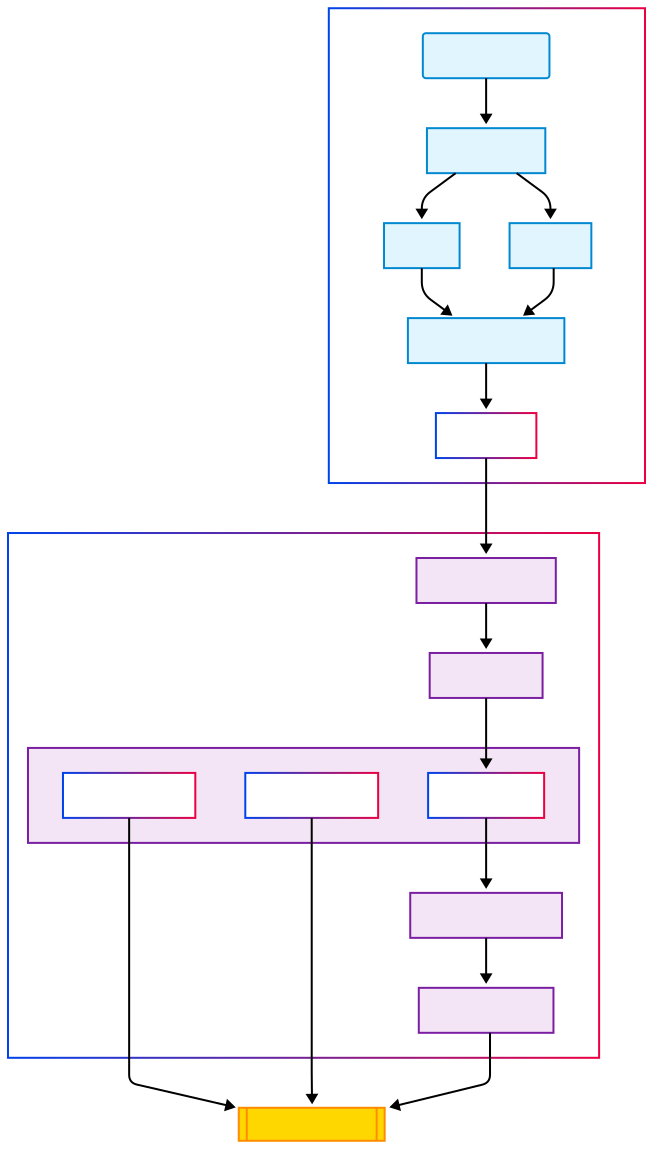
\includegraphics[width=0.85\textwidth]{img/user-diagram-flow}
\caption{High level workflow showing user interaction and data processing}
  \label{fig:user-flow}
\end{figure}

Next.js was chosen because it provides server-side rendering, built-in API routes, and excellent developer experience for building interactive applications. The App Router in Next.js 15 makes it easy to organize different parts of the application (dashboard, pitch pages, authentication) while maintaining clean code structure. This architecture supports the route groups used in the implementation, including `(dashboard)`, `(pitch)`, and `(auth)` directories that separate functional areas without affecting URL routing.

For the backend, Convex was selected after comparing it with traditional databases like PostgreSQL and other backend-as-a-service options. Convex provides real-time data synchronization, built-in schema validation, and server functions that run in the cloud. This eliminates the complexity of managing database connections, implementing real-time updates, or handling server deployment, allowing focus on the evaluation logic.

The authentication layer uses Clerk, which provides complete user management including organizations for multi-tenant data separation. This is important for research applications where different groups need to maintain separate data while using the same system. Clerk handles user registration, login, password management, and organization membership without requiring custom authentication logic.

For GenAI processing, OpenAI's GPT-4 API is used for all evaluation tasks and Whisper for audio transcription. This single-provider approach was chosen after testing multiple alternatives, as it provides the most consistent results while keeping the architecture simple. The system uses GPT-4 for structured evaluation, question generation, and answer processing, while Whisper handles audio file transcription with support for multiple audio formats.

\subsection{Evaluation Framework}\label{subsec:evaluation-framework}

The evaluation framework, developed by analyzing venture capital research and startup success factors, serves as the core mechanism for how Pista assesses startup pitches by identifying the most important evaluation criteria. The framework evaluates pitches systematically across multiple dimensions using standardized criteria and weighted scoring to ensure consistent assessments.

The framework evaluates pitches across four main dimensions, each with specific weights based on their importance for startup success:

\begin{itemize}
  \item \textbf{Problem\mbox{-}Solution Fit}: 0.3
  \item \textbf{Business Model \& Market}: 0.3
  \item \textbf{Team \& Execution}: 0.25
  \item \textbf{Pitch Quality}: 0.15
\end{itemize}

The highest weights were assigned to Problem-Solution Fit and Business Model \& Market because research consistently shows these factors are the strongest predictors of startup success. Team \& Execution receives the next highest weight since execution capability is crucial for converting good ideas into successful businesses. Pitch Quality has the lowest weight because while presentation skills matter for raising capital, they are less predictive of actual business outcomes.

Each dimension evaluates five specific aspects, creating a comprehensive 20-aspect evaluation framework. For example, Problem-Solution Fit examines problem definition clarity, solution innovation, market understanding, competitive advantage, and value proposition. This systematic breakdown ensures thorough coverage of all critical elements.

Figure~\ref{fig:eval-flow} illustrates how each pitch moves through the evaluation pipeline. The system analyzes the content against each dimension's criteria using GPT-4, then combines the results using the predetermined weights to calculate final scores.

\begin{figure}[H]
  \centering
  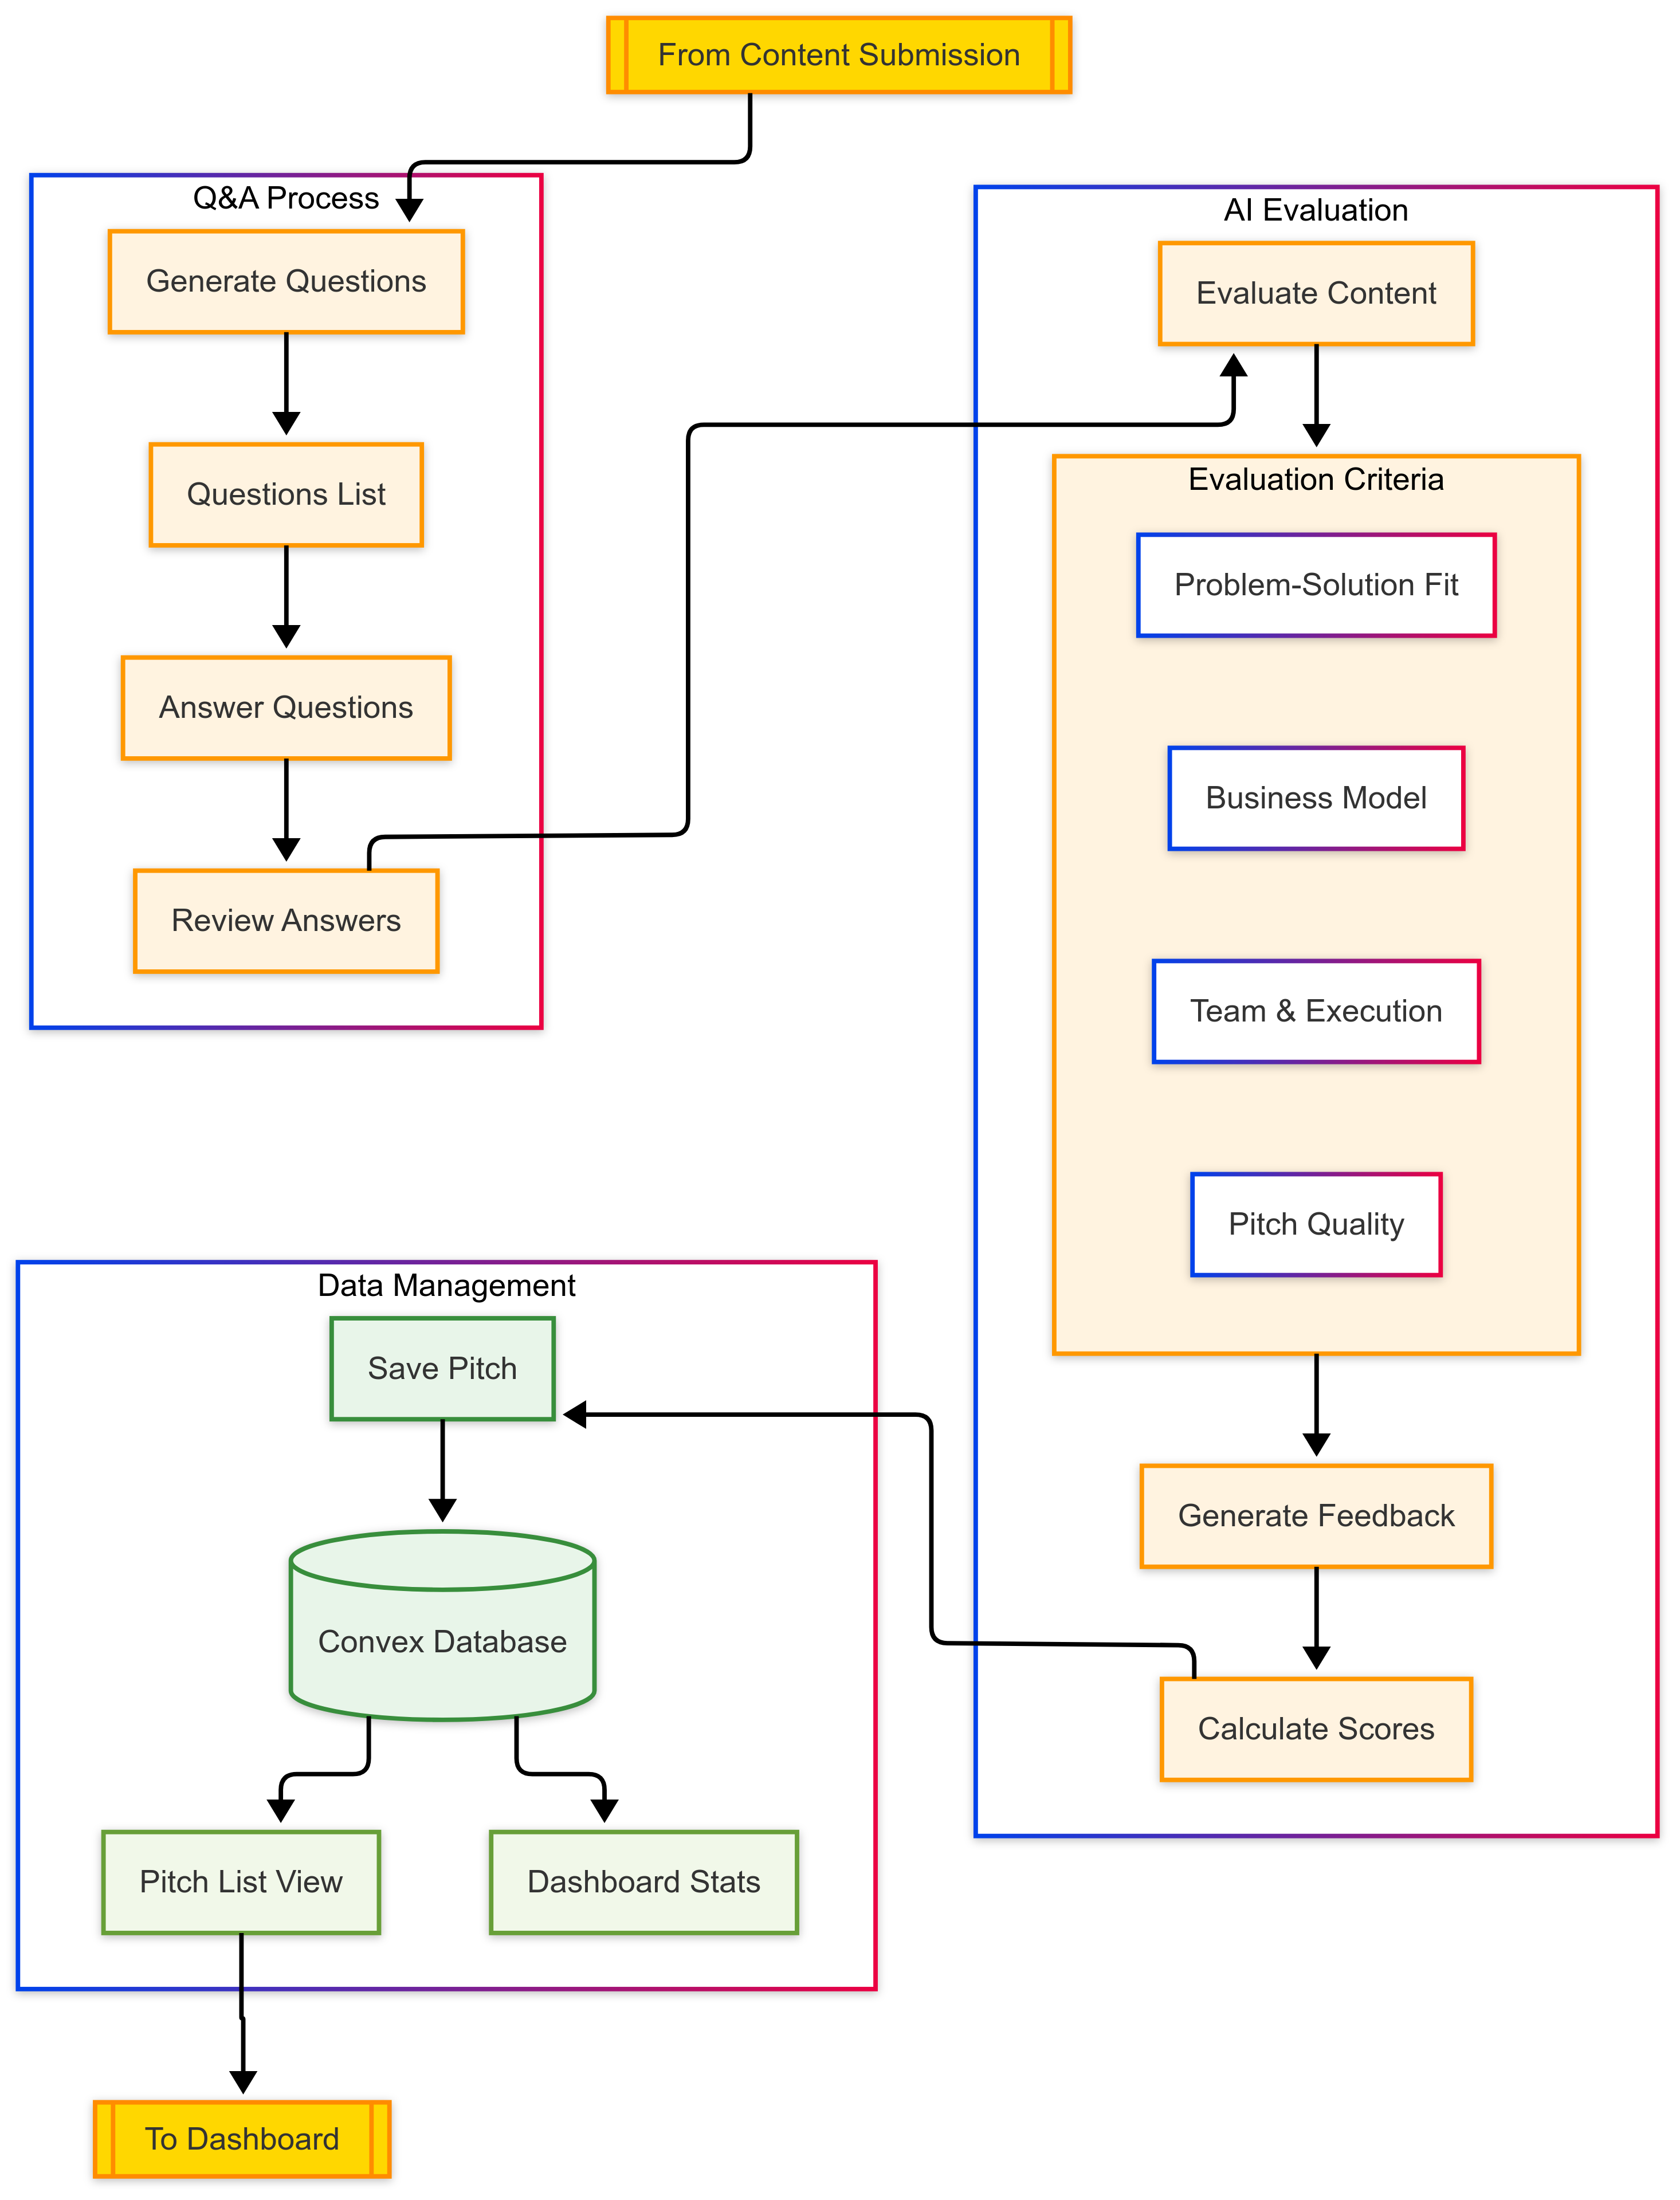
\includegraphics[width=0.9\textwidth]{img/eval-flow}
\caption{Evaluation and processing flow across four criteria}
  \label{fig:eval-flow}
\end{figure}

The scoring system uses a 1-10 scale with specific rubric anchors to ensure consistent evaluation; evidence-based scoring rules were implemented to prevent pitches from receiving high scores without supporting data. The rubric anchors define clear requirements for each score level:

\begin{enumerate}
    \item \textbf{Scores 1--2}: No concrete evidence, claims only
    \item \textbf{Scores 3--4}: Weak or indirect evidence, plan not validated
    \item \textbf{Scores 5--6}: Mixed evidence, partial validation or unclear metrics
    \item \textbf{Scores 7--8}: Strong evidence, credible metrics, risks addressed
    \item \textbf{Scores 9--10}: Exceptional evidence, repeated traction, benchmarks exceeded
\end{enumerate}

This evidence-gating approach addresses the central tendency problem where evaluations cluster around mid-scale scores without meaningful discrimination between pitch quality levels. The rubric was developed through iterative testing to ensure scores reflect actual business validation rather than presentation quality alone. These scoring rules prevent unsupported claims from receiving high ratings while rewarding pitches with concrete evidence of market traction and business validation.

Listing~\ref{lst:eval-criteria} shows how the evaluation criteria and weights were implemented as TypeScript constants to ensure consistency across all assessments.

\begin{lstlisting}[
  language=TypeScript,
  caption={Evaluation criteria and weights implementation},
  label=lst:eval-criteria,
  basicstyle=\footnotesize\ttfamily,
  breaklines=true
]
const EVALUATION_CRITERIA = {
  problemSolution: {
    name: "Problem-Solution Fit",
    aspects: [
      "Problem Definition Clarity",
      "Solution Innovation",
      "Market Understanding",
      "Competitive Advantage",
      "Value Proposition",
    ],
  },
  businessModel: {
    name: "Business Model & Market",
    aspects: [
      "Revenue Model",
      "Market Size & Growth",
      "Go-to-Market Strategy",
      "Customer Acquisition",
      "Scalability Potential",
    ],
  },
  team: {
    name: "Team & Execution",
    aspects: [
      "Team Capability",
      "Domain Expertise",
      "Track Record",
      "Resource Management",
      "Implementation Plan",
    ],
  },
  presentation: {
    name: "Pitch Quality",
    aspects: [
      "Clarity & Structure",
      "Data & Evidence",
      "Story & Engagement",
      "Q&A Performance",
      "Overall Persuasiveness",
    ],
  },
} as const;

const WEIGHTS: Record<string, number> = {
  "Problem-Solution Fit": 0.3,
  "Business Model & Market": 0.3,
  "Team & Execution": 0.25,
  "Pitch Quality": 0.15,
};
\end{lstlisting}

This implementation ensures every evaluation follows exactly the same criteria and weighting scheme. The criteria are defined as constants to prevent runtime modifications and maintain evaluation consistency. The TypeScript type system enforces proper usage of these constants throughout the codebase, preventing inadvertent changes to evaluation criteria during development.

\clearpage
\subsection{GenAI Integration Strategy}\label{subsec:genai-integration-strategy}

GPT-4 was integrated as the core evaluation engine after systematic testing showed it provided the most consistent and high-quality assessments. The integration uses structured prompts that return constrained JSON responses, ensuring reliable data parsing and consistent formatting. All API interactions include strict JSON schema validation to prevent malformed responses from corrupting evaluation data.

The prompt engineering process involved several iterations to optimize evaluation quality. Early testing identified a central tendency problem, where evaluations clustered around 7 out of 10, failing to discriminate between pitches of different quality levels. This was solved by implementing evidence-based scoring rules and rubric anchors.

Listing~\ref{lst:main-eval-prompt} shows the main evaluation prompt template that was developed for structured assessment:

\begin{lstlisting}[
  language=TypeScript,
  caption={Main evaluation prompt template for structured assessment},
  label=lst:main-eval-prompt,
  basicstyle=\footnotesize\ttfamily,
  breaklines=true
]
function buildStructuredPrompt(
  criteriaName: string,
  aspects: string[],
  fullContent: string
): string {
  return `
As an expert evaluator, score ONLY the criterion: ${criteriaName}.

Work from the content below without inventing facts. If evidence is
missing for an aspect, score that aspect <= 4 and note what is missing.

Aspects to score (each 1-10 with a one sentence rationale):
${aspects.map((aspect) => `- ${aspect}`).join("\n")}

Content to evaluate (pitch + Q&A):
${fullContent}

${RUBRIC_ANCHORS}

JSON response schema (valid JSON only):
{
  "score": 1-10, // criterion score = rounded average of aspectScores[].score
  "strengths": [{ "point": "...", "impact": "High"|"Medium"|"Low"}],
  "improvements": [{ "area": "...", "priority": "Critical"|"Important"|"Nice to Have", "actionable": "..."}],
  "aspectScores": [
    { "aspect": "${aspects[0]}", "score": 1-10, "rationale": "..." },
    { "aspect": "${aspects[1]}", "score": 1-10, "rationale": "..." },
    { "aspect": "${aspects[2]}", "score": 1-10, "rationale": "..." },
    { "aspect": "${aspects[3]}", "score": 1-10, "rationale": "..." },
    { "aspect": "${aspects[4]}", "score": 1-10, "rationale": "..." }
  ],
  "summary": "2-3 sentence synthesis",
  "recommendations": ["actionable step 1", "actionable step 2"]
}

${SCORING_RULES}
`;
}
\end{lstlisting}

This prompt template enforces evidence-based evaluation by explicitly instructing the model to avoid inventing facts and to cap scores at 4 when supporting evidence is missing. The structured JSON response ensures consistent data format across all evaluations.

A separate question generation system was also implemented to identify information gaps in pitch content. This system analyzes the pitch and generates up to 3 targeted questions that would materially improve evaluation quality if answered. The questions focus on specific evidence gaps that prevent confident evaluation rather than general business development advice.

\clearpage
Listing~\ref{lst:question-prompt} shows the question generation prompt:

\begin{lstlisting}[
  language=TypeScript,
  caption={Question generation prompt for evidence gathering},
  label=lst:question-prompt,
  basicstyle=\footnotesize\ttfamily,
  breaklines=true
]
const prompt = [
  `Analyze the following pitch and identify the most important gaps that prevent a confident evaluation. Select up to 3 questions that, if answered, would materially improve the assessment.`,
  `Pitch:\n"${truncate(text, MAX_PROMPT_CHARS)}"`,
  `\nReturn valid JSON only with this schema:\n{\n  "items": [\n    {\n "dimension": "Problem-Solution Fit" | "Business Model & Market" | "Team & Execution" | "Pitch Quality",\n      "question": "one specific question, no multi-part prompts",\n      "why_needed": "why this matters for evaluation",\n      "suggested_format": "how to answer: numbers, metrics, bullets, examples",\n      "priority": "Critical" | "Important"\n    }\n  ]\n}\n\nConstraints:\n- Ask 1-3 questions total.\n- Make each question specific and evidence-seeking.\n- Do not request sensitive data.\n- Avoid duplicates and multi-part questions.`,
].join("\n\n");
\end{lstlisting}


This question generation approach systematically identifies evidence gaps before conducting the final assessment, improving evaluation accuracy while ensuring questions remain answerable within a typical pitch context. The system constrains questions to avoid requesting sensitive data or internal documentation that would not be available in standard pitch scenarios. Each generated question includes priority levels and suggested answer formats to guide users toward providing the most valuable additional information for evaluation improvement.

For reliability, exponential backoff retries were implemented for API interactions and strict JSON validation before data persistence. The system uses a low temperature setting (0.2) for all evaluation requests to reduce randomness while maintaining appropriate response variation. Error handling includes comprehensive logging for debugging while ensuring user-facing error messages remain clear and actionable without exposing system internals.

\subsection{Data Models and Storage Architecture}\label{subsec:data-models-and-storage-architecture}

The data architecture was designed to support both real-time user interactions and research data collection. Convex combines database functionality with built-in schema validation and real-time synchronization. Convex provides automatic schema enforcement and type safety that prevents data corruption while eliminating the need for separate database migration management.

The main data model centers around the \texttt{`pitches`} table, which stores essential pitch information including title, content, submission type, processing status, structured evaluation results, question-answer pairs, and organizational metadata. Each document is automatically scoped by user and organization identifiers, providing secure data isolation for multi-tenant use.

The database schema implements several indexes to optimize query performance: \texttt{`by\_org`}, \texttt{`by\_user`}, \texttt{`by\_user\_org`}, and \texttt{`search\_title`}. The data model stores both structured evaluation results and complete audit trails for research reproducibility. Question-and-answer pairs are stored with each pitch and reused when building evaluation input, allowing systematic gathering of additional context that improves assessment quality. The system stores structured evaluation data with detailed scoring breakdowns and improvement recommendations for comprehensive analysis.

\subsection{API Endpoints and Server Functions}\label{subsec:api-and-server}

The API architecture uses Next.js API routes for GenAI processing and Convex functions for data management. This separation allows each component to be optimized for its specific computational requirements. Next.js API routes handle external integrations with OpenAI, while Convex functions manage all database operations with built-in real-time synchronization.

The GenAI processing endpoints include:
\begin{itemize}
  \item \texttt{/api/evaluate}: Processes pitch text using GPT-4 for comprehensive evaluation
  \item \texttt{/api/generate-questions}: Produces targeted follow-up questions using evidence-gap analysis
  \item \texttt{/api/transcribe}: Handles audio file transcription using OpenAI's Whisper model
  \item \texttt{/api/evaluate-answers}: Supports evaluation updates based on question responses
\end{itemize}

These endpoints run on Vercel's Edge runtime for improved performance and global distribution. All API responses are validated against strict schemas before data persistence to ensure research data integrity.

The Convex functions handle all data lifecycle operations including create, update, remove, favorite, unfavorite, and export operations. Query functions support diverse access patterns needed for both user interface functionality and research data analysis, including filtered searches, statistics, and CSV export for external analysis.

\section{Authentication and Authorization Implementation}

The authentication system uses Clerk to provide complete user management with multi-tenant organization support. This design ensures secure data isolation between different research groups while maintaining a simple security model. The implementation includes Next.js middleware that protects dashboard routes and redirects unauthenticated users to the sign-in page. Security headers are applied to all responses through the middleware layer, providing additional protection against common web vulnerabilities. The Clerk integration handles user registration, login, password management, and organization membership without requiring custom authentication logic, reducing security risks while maintaining a professional user experience.


\section{User Interface Implementation}

The user interface was built using Next.js 15 with React 18 and Tailwind CSS to provide a responsive, modern experience optimized for research applications. The application was organized using route groups to separate functional areas: dashboard for pitch management, individual pitch pages for detailed evaluation views, and authentication areas.

Figure~\ref{fig:dashboard} shows the main dashboard interface, which provides an overview of all pitch submissions with evaluation scores, search and filtering capabilities, and direct access to detailed results.

\begin{figure}[H]
  \centering
  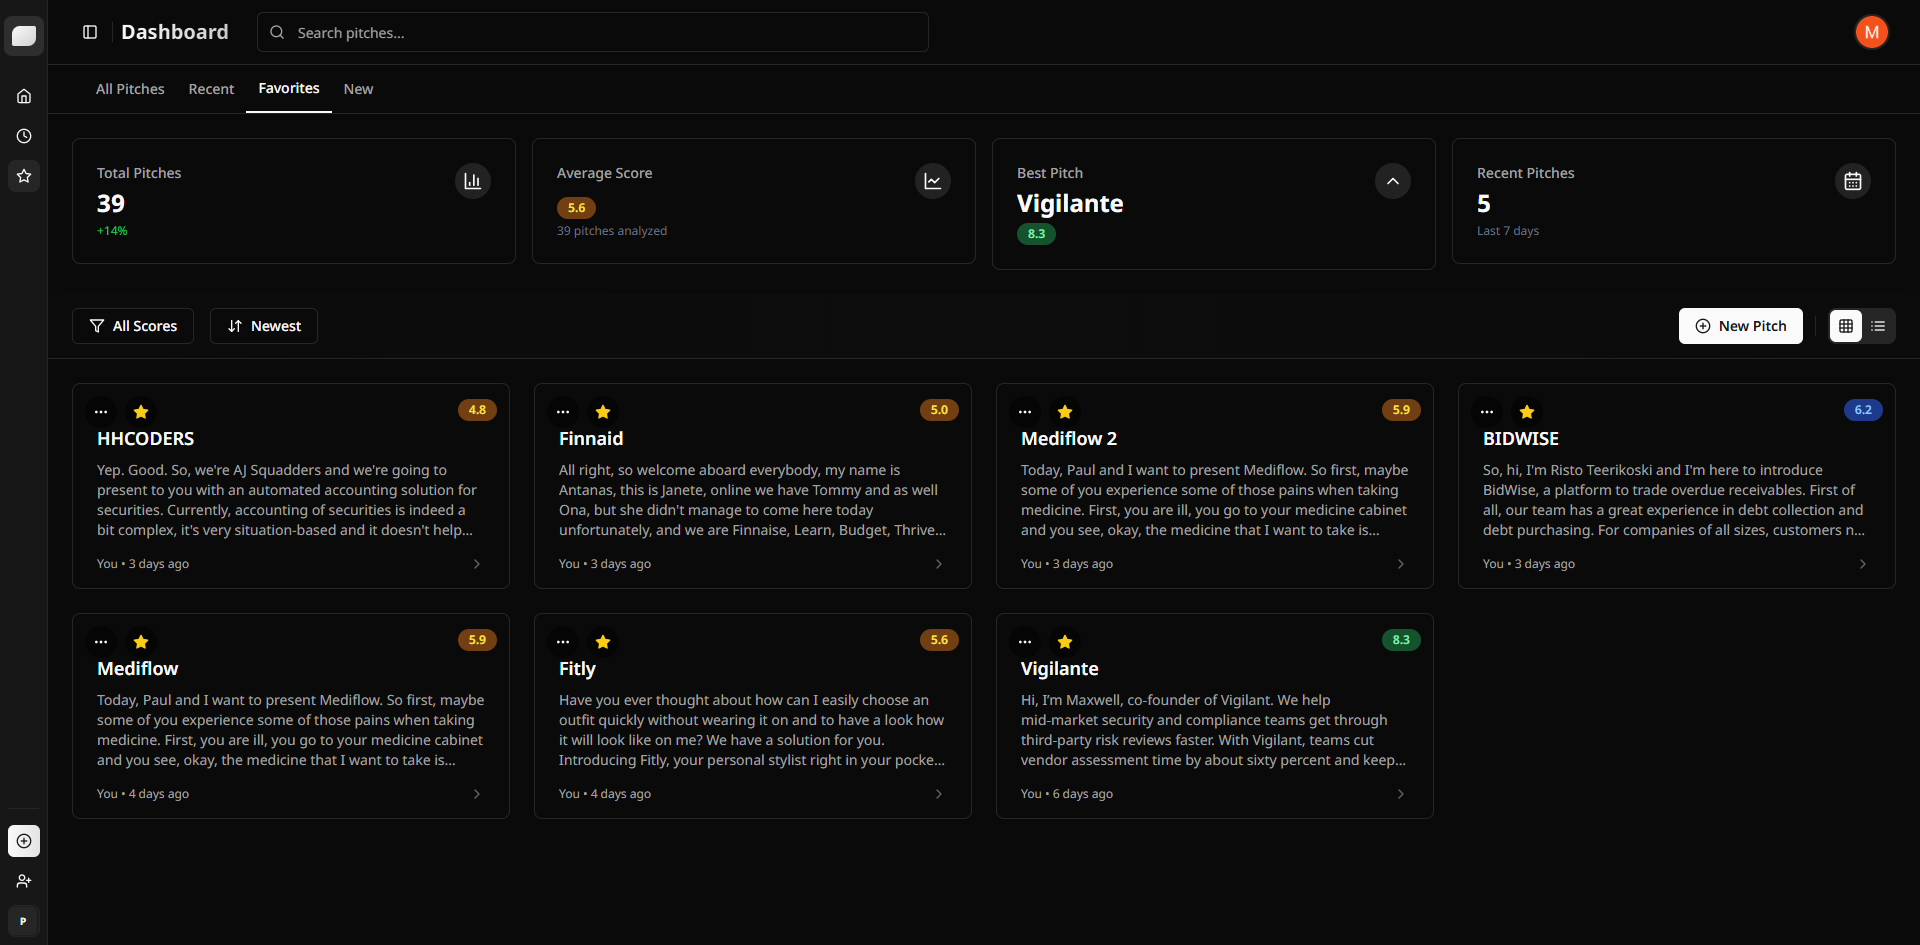
\includegraphics[width=0.9\textwidth]{img/dashboard}
\caption{Main dashboard interface showing pitch management and evaluation scores}
  \label{fig:dashboard}
\end{figure}

The component architecture separates shared UI primitives from feature-specific components to promote reusability and consistent design patterns. The dashboard implements comprehensive list management with user favorites, text-based search, and filtering by evaluation scores or submission dates. Components are organized into logical directories with 'src/components/ui/' containing base components and 'src/components/shared/' housing feature-specific components grouped by domain, including navigation, forms, modals, and authentication. The multi-step pitch upload process uses a dedicated component hierarchy in `src/components/shared/forms/add-pitches/steps/` that manages state progression, validation, and user guidance throughout the evaluation workflow. This architectural separation ensures consistent design language while enabling independent development and testing of complex features like the question generation and evaluation display components.

Figure~\ref{fig:user-flow-pitch} illustrates the pitch creation workflow that was designed to guide users through the evaluation process efficiently. The flow handles both text input and audio file uploads, manages question generation and response collection, and performs evaluation processing with complete metadata storage.

\begin{figure}[H]
  \centering
  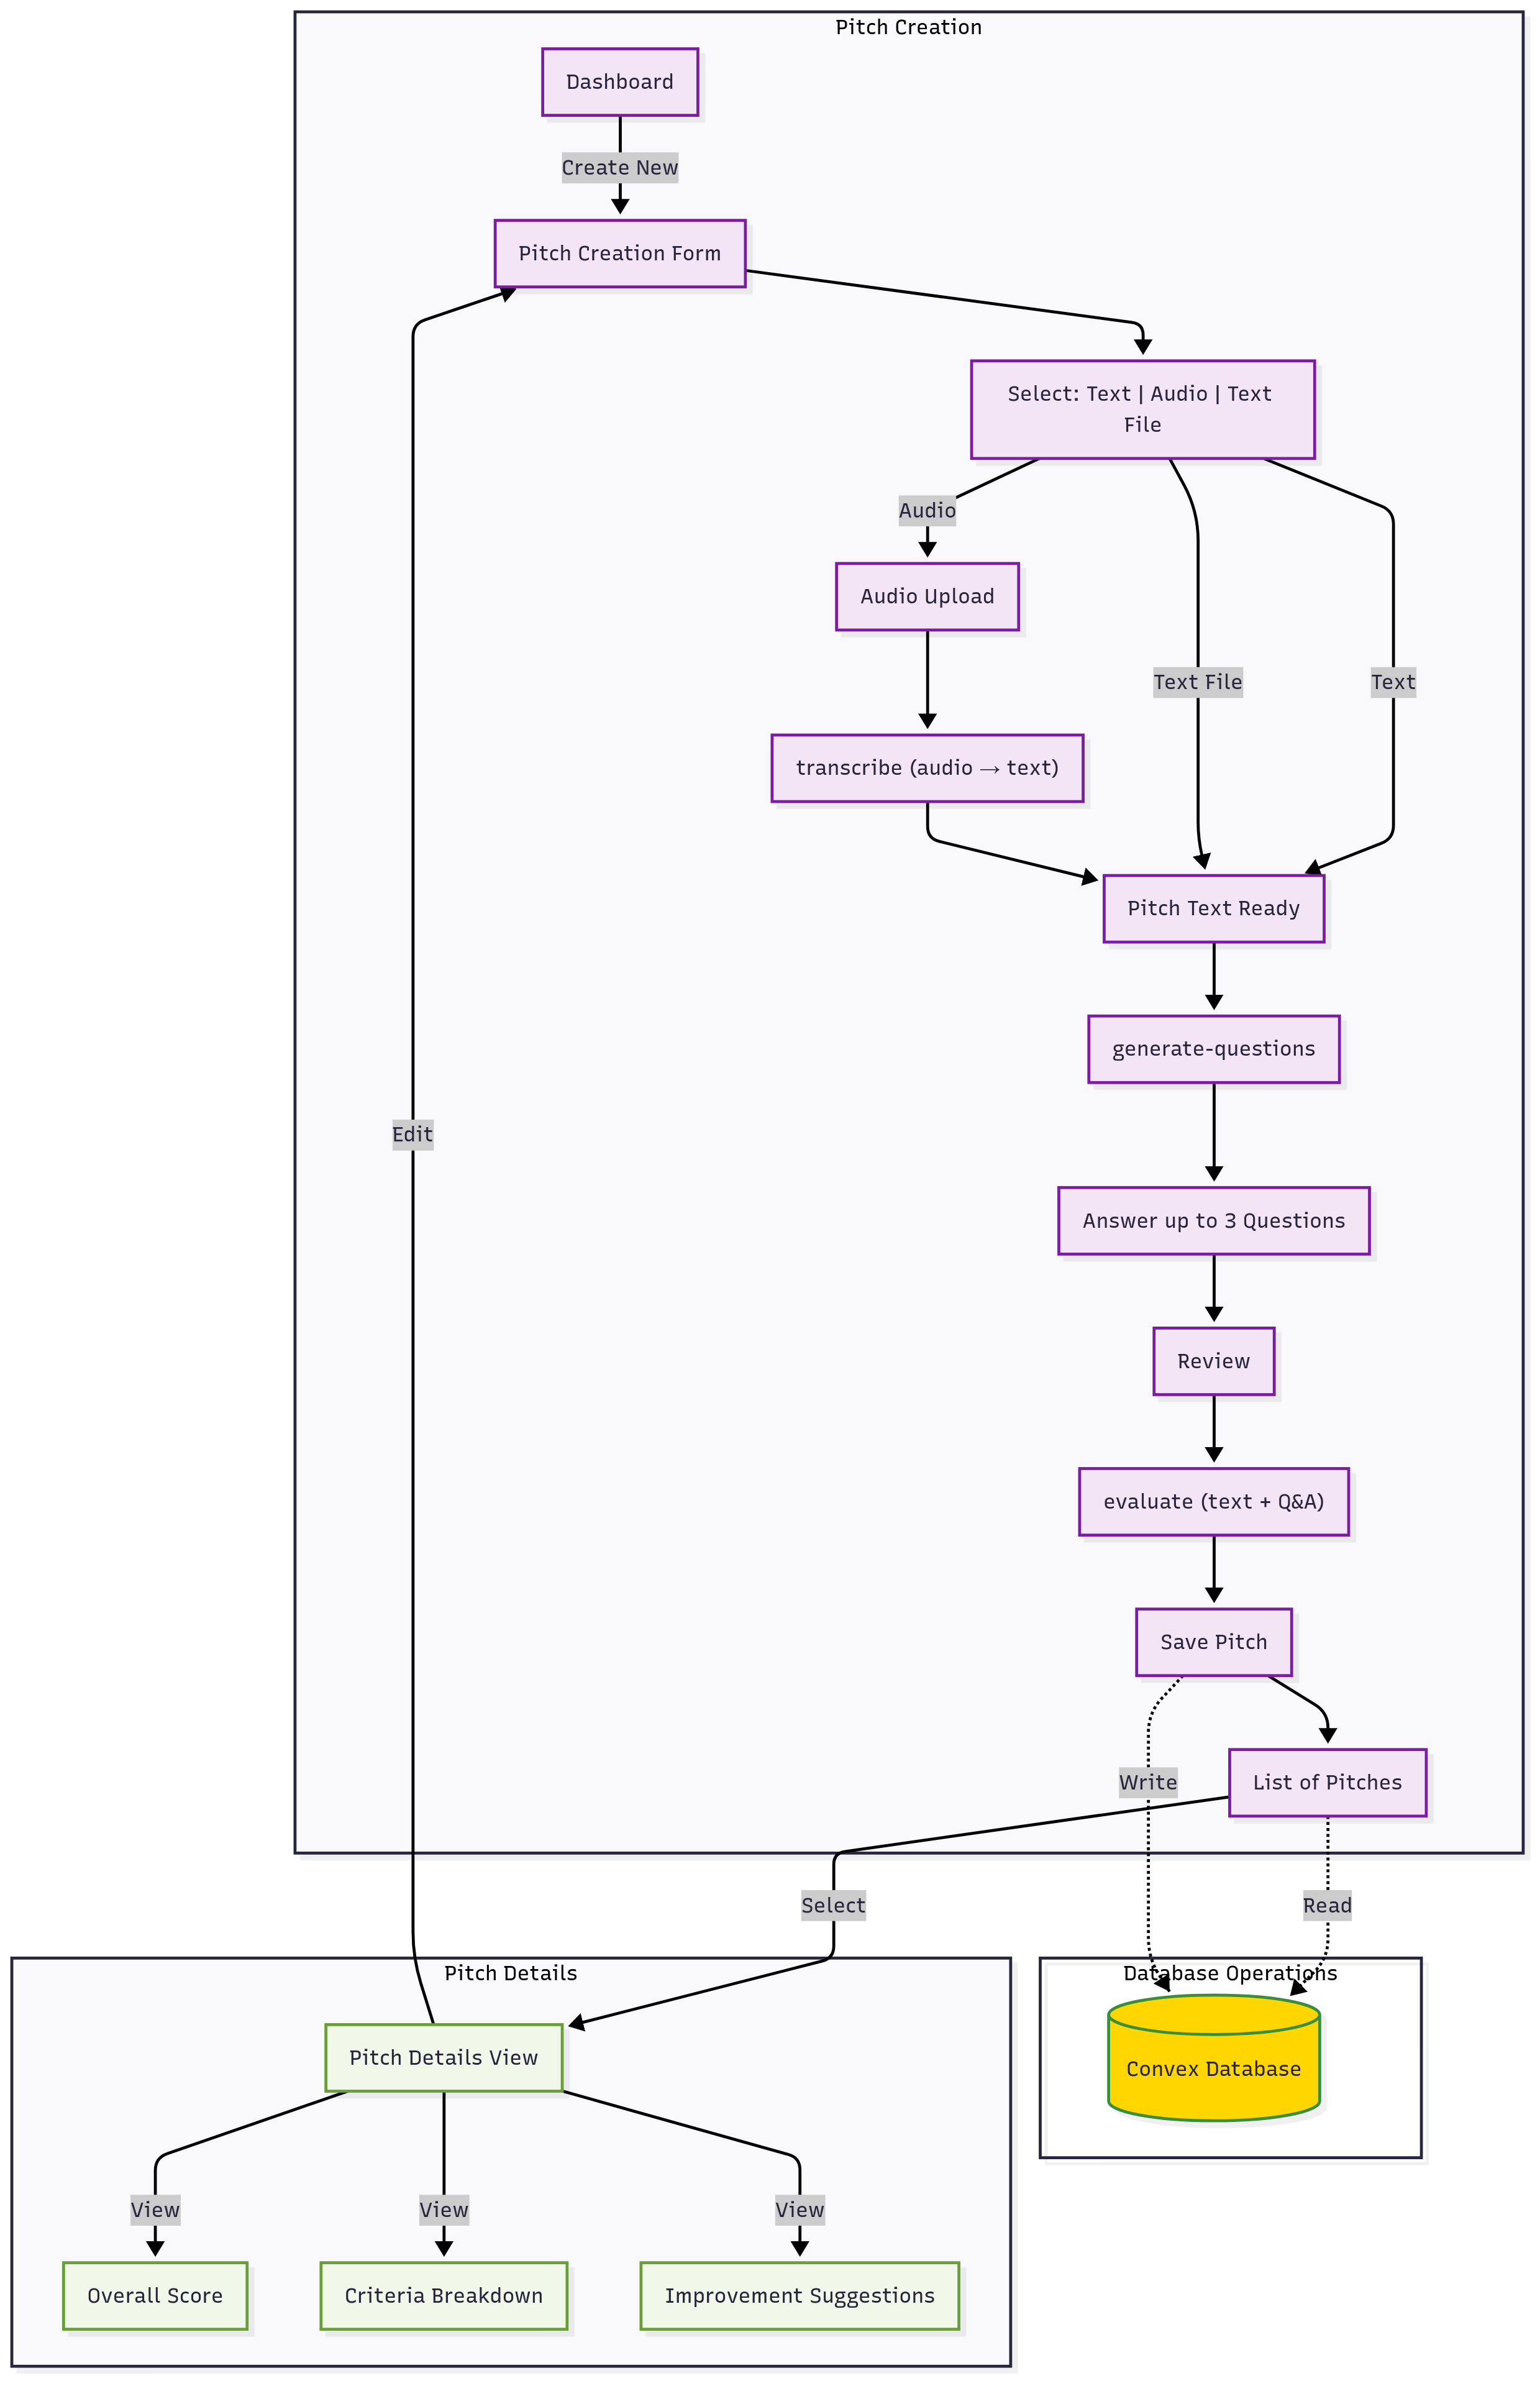
\includegraphics[width=0.9\textwidth]{img/user-flow-pitch}
\caption{Pitch creation flow with Q\&A generation and Convex storage}
  \label{fig:user-flow-pitch}
\end{figure}

The question-and-answer step is optional but enabled by default based on testing that showed significant evaluation quality improvements. Users can skip this step for faster processing, though this may result in less comprehensive evaluations when key information is missing from the original pitch. The questions component implements a multi-step interface that presents one question at a time with visual progress indicators, helping users maintain focus while providing targeted responses that address specific evaluation criteria gaps. The system dynamically generates up to three questions using GPT-4's analysis of the pitch content, with each question targeting critical missing information needed for accurate assessment. The component includes explanatory text stating ``\textit{These questions help improve your evaluation accuracy}'' to guide user understanding of the purpose and value of providing additional context during the evaluation process.

The individual pitch view renders both numeric scores and qualitative feedback alongside generated follow-up questions, providing users with complete evaluation information in a clear, structured format optimized for review and improvement planning. The pitch page implementation uses lazy loading to optimize performance by loading components such as `ScoreOverview`, `EvaluationSummary`, `DetailedAnalysis`, and `QuestionsSection` only when needed, while maintaining responsive skeleton placeholders during content loading. The system supports both legacy and structured evaluation formats through conditional rendering that automatically detects the evaluation data type and displays the appropriate analysis components. This modular architecture enables rich data visualization with transcript sections, comprehensive score breakdowns, and targeted improvement recommendations while maintaining fast initial page loads and smooth user interactions throughout the evaluation review process.

\section{Performance, Deployment, and Reliability}

System performance was optimized to handle the computational demands of GenAI processing while maintaining responsive user interactions. The implementation uses virtualized lists to maintain interface responsiveness with large datasets, code splitting to reduce initial page load times, and reactive queries that eliminate manual polling by automatically updating the interface when results become available.

The deployment architecture uses Vercel for hosting with environment variables for configuration, including database URLs, authentication keys, and API credentials. Critical API routes run on Vercel's Edge runtime for global distribution and reduced latency. The deployment pipeline ensures identical code paths across development and production environments to maintain evaluation result consistency.

For reliability, comprehensive error handling was implemented throughout the system. API routes return clear, actionable error messages that help users resolve problems without exposing sensitive system details. The system includes exponential backoff retries for external API interactions and strict JSON validation before data persistence to prevent corrupted evaluations from entering the research database.

\section{Implementation Results and User Experience}\label{sec:results}

The implemented system achieves the design goals of providing consistent, evidence-based startup pitch evaluations. Text-based pitch evaluations typically complete within 30 to 60 seconds, providing timely feedback without disrupting research workflows. Audio-based submissions require additional processing time for transcription but remain within acceptable bounds for practical use.

The user interface provides immediate visual feedback throughout the evaluation process with real-time updates that make data changes visible without manual page refreshes. The system maintains responsive performance during concurrent usage, supporting both individual use and classroom scenarios where multiple students submit pitches simultaneously.

The systematic development approach ensured all components integrate properly while maintaining research data integrity. The evidence-based evaluation framework successfully addresses the central tendency problem identified in initial testing, producing meaningful score distributions that discriminate between pitches of different quality levels.

The complete implementation represents a working system that combines GenAI capabilities with research-quality data collection, providing both immediate user value and a foundation for continued evaluation  research.
% chapters/4-evaluation.tex
\chapter{Evaluation and Results}
\label{ch:evaluation}

This chapter evaluates the Pista system by comparing it with Winds2Ventures (W2V)\footnote{\url{https://w2v.network/}}, an existing pitch evaluation platform. The comparison examines differences in scoring patterns and evaluation approaches between the GenAI-powered system and the established platform.

Evaluating startup pitches involves subjective judgment and domain expertise. To validate the Pista system, comparison with an existing evaluation platform provides insights into how GenAI approaches differ from human-driven assessment methods.

The comparison examined differences in scoring patterns, evaluation consistency, and assessment approaches between the two systems. The analysis focused on understanding where each system shows strengths and limitations.

Comparing GenAI evaluation with existing platforms helps understand the practical utility and limitations of automated assessment tools for startup pitch evaluation.

The comparison addressed three key questions:
\begin{enumerate}
    \item How do Pista scores compare with W2V assessments?
    \item What patterns emerge in the scoring differences?
    \item What are the practical implications for using GenAI evaluation tools?
\end{enumerate}

\section{Methodology and Experimental Design}
\label{sec:methodology}

All results in this chapter use the calibrated scoring prompt (\texttt{PROMPT\_VERSION = criteria\textrm{-}v1.2}) with rubric anchors, evidence gating, aspect first scoring, and a lower sampling temperature for scoring. When Q\&A is enabled, the question generator asks for 1--3 structured, evidence seeking questions and accepts JSON or a numbered list fallback.

\subsection{Metrics}
To evaluate distribution quality and alignment, the analysis reports:
\begin{itemize}
  \item \textbf{Score concentration}: share of exact 7.0 scores before/after calibration
  \item \textbf{Dispersion}: variance or IQR per criterion
  \item \textbf{Rank alignment}: Kendall's $\tau$ with baseline/commercial assessments
  \item \textbf{Evidence sensitivity}: proportion of scores $\leq 4$ when specific evidence is missing
\end{itemize}

\section{Future Work: Ensemble Evaluation}
The current implementation uses a single provider (GPT\,4) with rubric anchored prompts. A practical extension is an ensemble across multiple models to improve stability and evidence coverage:
\begin{itemize}
  \item \textbf{Providers}: Add adapters for OpenAI, Anthropic, and Google; run all providers per criterion in parallel.
  \item \textbf{Aggregation Policy}: Aggregate aspect scores via trimmed mean (e.g., 20\% trim if $\geq$3 providers), then average to the criterion score; record provenance.\footnote{Bump \texttt{POLICY\_VERSION} to \texttt{scoring-policy-v3}.}
  \item \textbf{Disagreement Flags}: If interquartile range across provider scores exceeds a threshold, mark the criterion as low confidence.
  \item \textbf{Adjudication (Optional)}: For flagged criteria, use an adjudicator prompt to merge rationales into the final JSON.
  \item \textbf{Disagreement-Driven Q\&A}: When flagged, generate 1--3 targeted questions for the highest-variance aspects and re-score on answers.
  \item \textbf{Reporting}: Compare ensemble vs. single provider on score dispersion and Kendall's $\tau$ against the baseline (W2V), and document cost/latency trade-offs.
\end{itemize}

\subsection{Dataset Selection and Characteristics}
\label{subsec:dataset}

Twenty-two startup pitches from university entrepreneurship competitions were evaluated by both systems. University competition pitches provided consistent content and format, enabling direct comparison between the two evaluation approaches.

Both systems evaluated all 22 pitches, covering diverse sectors including technology, healthcare, agriculture, and consumer services.

The pitches were obtained through university entrepreneurship programs with appropriate permissions for research use.

Each pitch contained the fundamental components required for comprehensive startup evaluation: clearly defined problem statements, proposed solution descriptions, market opportunity analysis, team capability presentations, and business model articulation. The standardized competition format ensured consistent information availability across all evaluated pitches, facilitating meaningful cross-system comparison.

\subsection{Evaluation Framework Comparison}
\label{subsec:frameworks}

Fundamental differences in evaluation architecture between the two systems necessitated careful methodological consideration for comparative analysis. Each platform employs distinct assessment criteria and weighting mechanisms that reflect different philosophical approaches to startup evaluation.

\subsubsection{Pista Evaluation Framework}

The Pista system employs a four-dimensional weighted assessment structure designed to capture critical aspects of startup viability. The dimensional weighting was calibrated based on venture capital research findings and established industry evaluation practices.

The assessment framework comprises four weighted dimensions:
\begin{enumerate}
    \item \textbf{Problem-Solution Fit (30\% weight)}: Examination of problem definition clarity, solution innovation depth, market understanding sophistication, competitive differentiation strength, and value proposition coherence.

    \item \textbf{Business Model \& Market (30\% weight)}: Analysis of revenue model sustainability, market size estimation credibility, go-to-market strategy feasibility, customer acquisition viability, and scalability potential.

    \item \textbf{Team \& Execution (25\% weight)}: Assessment of team competency profiles, domain expertise relevance, historical performance indicators, resource allocation efficiency, and implementation strategy depth.

    \item \textbf{Pitch Quality (15\% weight)}: Evaluation of presentation structure, evidence integration effectiveness, narrative coherence, and persuasive communication quality.
\end{enumerate}

Quantitative scores are generated on a standardized 1-10 scale for each dimension, accompanied by qualitative feedback containing specific improvement recommendations. The final assessment emerges through weighted aggregation of dimensional scores.

\subsubsection{Winds2Ventures Evaluation Framework}

The Winds2Ventures platform operates through a nine-criteria assessment methodology focused on investment readiness and commercial viability indicators. Each evaluation criterion contributes to an aggregate "Investibility" rating that reflects overall investment attractiveness from a professional investor perspective.

The evaluation criteria encompass:
\begin{enumerate}
    \item \textbf{Problem Clarity}: Assessment of problem definition precision and market relevance
    \item \textbf{Solution Viability}: Analysis of proposed solution feasibility and effectiveness potential
    \item \textbf{Market Size Estimation}: Evaluation of addressable market opportunity and growth projections
    \item \textbf{Competitive Advantages}: Examination of differentiation strategies and sustainable positioning
    \item \textbf{Team Assessment}: Analysis of team competencies, experience, and execution capabilities
    \item \textbf{Business Model Viability}: Investigation of revenue mechanisms and sustainability factors
    \item \textbf{Go-To-Market Strategy}: Review of market entry approaches and scaling methodologies
    \item \textbf{Competitive Landscape}: Assessment of market dynamics and competitive positioning
    \item \textbf{Funding Ask and Use}: Analysis of capital requirements and allocation strategies
\end{enumerate}

The W2V evaluation process involves experienced investors and business professionals who contribute extensive industry knowledge and practical investment experience. This human expertise emphasizes realistic market dynamics and execution risk factors, typically resulting in more conservative assessment patterns than algorithmic evaluation approaches.

\subsection{Score Mapping and Comparison Methodology}
\label{subsec:methodology-approach}

The divergent evaluation frameworks presented methodological challenges for direct comparative analysis. To address these complexities, a conservative analytical approach was adopted that focused primarily on overall assessment scores rather than attempting complex dimensional mappings between disparate criteria sets.

The comparison methodology centered on Pista's weighted overall scores against W2V's Investibility ratings. Both systems generate standardized 1-10 scale assessments, facilitating direct numerical comparison without requiring complex score transformations or normalization procedures. This approach preserved the integrity of each system's underlying evaluation philosophy while enabling meaningful quantitative analysis.

\section{Results and Analysis}
\label{sec:results}

\subsection{Overall Performance Patterns}
\label{subsec:performance}

The comparative analysis revealed systematic differences between evaluation systems that extend beyond random variation, suggesting fundamental divergences in assessment philosophy and methodology. These patterns emerged consistently across all evaluated pitches, indicating structural rather than circumstantial differences.

Across all 22 evaluated pitches, Pista consistently generated higher scores than W2V, with no exceptions observed. The average scoring differential measured +1.70 points, representing a substantial and systematic bias that suggests underlying philosophical differences in evaluation approach rather than random measurement variation.

\begin{table}[ht]
    \centering
    \caption{Comprehensive Score Comparison Analysis}
    \label{tab:score-comparison}
    \begin{tabular}{lccc}
        \toprule
        \textbf{System} & \textbf{Average Score} & \textbf{Score Range} & \textbf{Standard Deviation} \\
        \midrule
        Pista & 6.81/10 & 6.0-8.0 & 0.50 \\
        Winds2Ventures & 5.11/10 & 4.3-6.4 & 0.63 \\
        \midrule
        \textbf{Difference} & +1.70 & - & - \\
        \bottomrule
    \end{tabular}
\end{table}

Analysis of scoring distributions revealed significant differences in discrimination capabilities between the evaluation systems.

Pista scores demonstrated clustering within a relatively narrow 6.0-8.0 range, producing a standard deviation of 0.50. In contrast, W2V scores exhibited broader distribution spanning 4.3-6.4 points with higher variance ( = 0.63). These distribution patterns suggest different approaches to quality discrimination, with W2V demonstrating greater sensitivity to quality variations across evaluated pitches.

\subsection{Systematic Bias Identification}
\label{subsec:bias}

Detailed pattern analysis exposed several consistent systematic biases that significantly influence GenAI evaluation reliability and practical deployment viability.

\subsubsection{Systematic Optimism Bias}

The most prominent bias emerged as universal optimism in GenAI scoring patterns. Across all 22 evaluated pitches, Pista consistently generated higher scores than W2V without exception. This universal directional bias transcended pitch quality variations and industry sectors, suggesting systematic rather than circumstantial influences.

Several factors likely contribute to this optimism bias. Training data composition may overrepresent successful startup examples, creating algorithmic tendencies toward positive assessment. Additionally, GenAI systems may lack the sophisticated risk evaluation capabilities that characterize experienced human evaluators, who integrate market realities and execution challenges developed through practical investment experience.

\subsubsection{Limited Discriminative Power}

A striking pattern emerged in score distribution analysis: 66.7\% of Pista evaluations (15/22 pitches) received identical overall scores of exactly 7.0/10. This substantial clustering indicates critical algorithmic limitations in quality differentiation capabilities. Rather than reflecting genuine quality similarities among evaluated pitches, this pattern suggests algorithmic convergence toward a default "safe" assessment value.

Such limited discrimination presents significant challenges for practical investment applications. Professional investors require granular quality distinctions to effectively prioritize opportunities and allocate limited evaluation resources. When most assessments converge on identical scores, the system fails to provide the nuanced discrimination essential for informed decision-making.

\begin{table}[ht]
    \centering
    \caption{Systematic Bias Analysis}
    \label{tab:bias-analysis}
    \begin{tabular}{lccc}
        \toprule
        \textbf{Bias Category} & \textbf{Frequency} & \textbf{Impact Magnitude} & \textbf{Strategic Implications} \\
        \midrule
        GenAI Evaluation Optimism & 22/22 (100\%) & +1.70 points average & Systematic over-confidence \\
        Limited GenAI Discrimination & 15/22 (66.7\%) & Identical scores & Insufficient quality differentiation \\
        Commercial Conservatism & 22/22 (100\%) & Consistent lower scoring & Risk-aware assessment \\
        \bottomrule
    \end{tabular}
\end{table}

\subsection{Dimensional Performance Analysis}
\label{subsec:dimensional}

\begin{table}[ht]
    \centering
    \caption{Pista Dimensional Performance Analysis}
    \label{tab:dimensional-analysis}
    \begin{tabular}{lcc}
        \toprule
        \textbf{Dimension} & \textbf{Pista Average} & \textbf{Performance Characteristics} \\
        \midrule
        Problem-Solution Fit & 7.1/10 & Highest dimensional performance \\
        Business Model \& Market & 6.9/10 & Consistently strong assessment \\
        Pitch Quality & 6.8/10 & Stable evaluation patterns \\
        Team \& Execution & 6.6/10 & Comparatively lower performance \\
        \bottomrule
    \end{tabular}
\end{table}

Dimensional analysis exposed systematic performance variations across evaluation categories, revealing specific algorithmic strengths and limitations. Problem-Solution Fit achieved the highest average scores (7.1/10), suggesting that GenAI systems demonstrate particular effectiveness in analyzing business logic structures and solution viability assessments.

Conversely, Team \& Execution consistently received the lowest dimensional scores (6.6/10), indicating algorithmic challenges in assessing human capital factors. This performance gap likely reflects GenAI limitations in evaluating intangible elements such as leadership depth, team dynamics, and execution track records—factors that human evaluators assess through experience-based pattern recognition and interpersonal judgment.

\section{Case Study Analysis}

\begin{table}[ht]
    \centering
    \caption{Comparative Case Study Analysis}
    \label{tab:case-studies}
    \begin{tabular}{lp{3cm}cccp{4cm}}
        \toprule
        \textbf{Company} & \textbf{Description} & \textbf{Pista Score} & \textbf{W2V Score} & \textbf{Difference} & \textbf{Primary Evaluation Focus Difference} \\
        \midrule
        Coontent & Marketing automation B2B SaaS platform & 6.5/10 & 5.3/10 & +1.2 & GenAI: Innovation potential vs W2V: Market competition \\
        \midrule
        Serenity & GenAI-powered mental wellness platform & 6.9/10 & 6.1/10 & +0.8 & GenAI: Market opportunity vs W2V: Regulatory challenges \\
        \midrule
        CampoRapido & Agricultural technology platform & 7.0/10 & 4.5/10 & +2.5 & GenAI: Problem-solution fit vs W2V: Market readiness \\
        \midrule
        Corptech & Industrial technology platform & 8.0/10 & 6.0/10 & +2.0 & GenAI: Technical innovation vs W2V: Execution readiness \\
        \bottomrule
    \end{tabular}
\end{table}

Case study analysis across diverse industry sectors revealed three distinct patterns that illuminate fundamental evaluation differences. First, scoring differentials ranged from 0.8 to 2.5 points, with regulated industries (Serenity: +0.8) showing smaller gaps and agricultural technology (CampoRapido: +2.5) exhibiting the largest disparities. Second, evaluation focus differed systematically: Pista emphasized innovation potential and technical merit, while W2V prioritized practical deployment challenges including regulatory compliance, market readiness, and execution risks. Third, even high-performing pitches like Corptech, which received the highest scores from both systems (8.0 Pista, 6.0 W2V), maintained substantial scoring gaps (+2.0), confirming that evaluation differences stem from systematic philosophical divergences rather than pitch quality variations.

\section{Discussion and Deployment Implications}

The comparison revealed consistent differences between Pista and W2V scoring approaches. Pista scored higher in all cases (100\% of cases, +1.70 average difference), suggesting the GenAI system tends toward more optimistic assessments than the W2V platform.

A notable finding is the limited score variation in Pista: 66.7\% of evaluations received identical 7.0/10 scores, while W2V showed more varied scoring across a 2.1-point range. This suggests the GenAI system tends toward consistent scoring rather than discriminating between different quality levels.

\subsection{Systematic Bias Analysis}
\label{sec:bias-analysis}

The comparison reveals three main patterns in how Pista differs from W2V in its evaluation approach.

\subsubsection{Universal GenAI Optimism}
\label{subsec:optimism}

Pista's consistent higher scoring (22/22 pitches) was interpreted as suggesting a training bias toward positive examples; it was also considered to indicate insufficient risk assessment capabilities. This optimism was identified as limiting utility for investment decision contexts.

The universal directional bias indicates that GenAI systems may be fundamentally designed to highlight opportunities rather than assess risks. This could result from training data that emphasizes successful startup characteristics without adequate representation of failure patterns. Commercial evaluators, by contrast, integrate market realities and execution challenges that create more conservative assessments.

\subsubsection{Score Convergence Limitations}
\label{subsec:convergence}

The concentration of 66.7\% of scores at exactly 7.0/10 was identified as indicating critical algorithmic limitations in quality differentiation. This clustering was interpreted as suggesting the evaluation model defaults to a "safe" middle-high score regardless of actual pitch quality variations.

This convergence pattern creates several practical challenges. Investment decisions require discrimination between opportunities to allocate resources effectively. When most evaluations receive identical scores, the system fails to provide the granular assessment needed for professional deployment. The algorithmic tendency toward convergence may reflect conservative design choices that prioritize consistency over discrimination.

\subsubsection{Risk Assessment Variations}
\label{subsec:risk}

Maximum disagreements occurred in technology and service platforms where commercial evaluators emphasized execution risks and market competition factors that GenAI evaluation appears to underweight.

GenAI systems focus on innovation potential and technical merit while underweighting execution challenges and competitive dynamics. Commercial platforms incorporate broader risk factors developed through investment experience. This difference reflects fundamental evaluation philosophy variations rather than calibration issues.

\subsection{Deployment Strategy Implications}
\label{sec:deployment}

The systematic differences suggest complementary rather than competing deployment strategies. Given GenAI's operational advantages (speed, cost, accessibility) and limitations (optimism bias, poor discrimination), strategic deployment becomes crucial.

\subsubsection{Appropriate GenAI Applications}
\label{subsec:ai-applications}

GenAI evaluation systems demonstrate clear advantages for specific use cases that align with their operational strengths and philosophical characteristics:

\textbf{Early-stage entrepreneur feedback and pitch development support}: The systematic optimism bias becomes advantageous for encouraging entrepreneurs and providing constructive feedback without discouraging innovation attempts.

\textbf{High-volume initial screening where broad categorization suffices}: The speed and cost advantages enable processing large numbers of pitches where precise discrimination is less critical than general quality assessment.

\textbf{Educational contexts where encouraging feedback promotes learning}: The consistent scoring patterns provide stable feedback that supports learning environments without creating discouraging assessment variations.

\subsubsection{Commercial Evaluation Requirements}
\label{subsec:commercial-requirements}

Commercial evaluation platforms demonstrate capabilities that remain essential for professional investment contexts:

\textbf{Investment decision-making requiring realistic risk assessment}: The broader score distribution and conservative assessment approach align with professional investment requirements for risk evaluation.

\textbf{Applications demanding granular quality discrimination}: The varied scoring patterns enable the discrimination needed for resource allocation and opportunity prioritization in competitive markets.

\textbf{Complex market sectors}: Technology and B2B services may benefit from the domain expertise that platforms like W2V provide through experienced evaluators.

\subsubsection{Hybrid Strategy Optimization}
\label{subsec:hybrid}

Using GenAI tools like Pista for initial feedback and platforms like W2V for more detailed assessment could combine the speed of GenAI with the nuanced evaluation of experienced assessors.

The hybrid strategy addresses both system limitations and advantages. GenAI systems handle high-volume screening efficiently while commercial systems provide the discrimination and risk assessment needed for investment decisions. This complementary approach maximizes overall evaluation system effectiveness.

\subsection{Evaluation Quality vs. Operational Efficiency Trade-offs}
\label{sec:tradeoffs}

The evaluation reveals a fundamental trade-off between operational efficiency and assessment quality. GenAI evaluation provides substantial operational advantages but at the cost of evaluation precision and realistic risk assessment.

\subsubsection{Operational Advantages}
\label{subsec:advantages}

GenAI's speed (30-60 seconds), cost (\$0.10-0.15), and availability (24/7) enable applications impossible with traditional evaluation methods, democratizing access to startup feedback. These advantages create entirely new use cases that were previously economically unfeasible.

The operational efficiency enables applications such as real-time pitch feedback during development, continuous iteration support, and accessible evaluation for entrepreneurs who cannot afford professional assessment services. This democratization effect represents a significant value creation opportunity.

\subsubsection{Quality Limitations}
\label{subsec:limitations}

The 66.7\% score convergence and systematic optimism bias severely limit GenAI utility for contexts requiring discriminative assessment or realistic risk evaluation. These limitations constrain professional deployment opportunities where quality assessment is critical.

The quality limitations become particularly problematic when AI evaluation results influence significant decisions. Investment contexts require accurate risk assessment and quality discrimination that current GenAI systems cannot provide reliably. This constrains professional deployment until these limitations are addressed.

\subsubsection{Strategic Trade-off Management}
\label{subsec:strategy}

These differences suggest GenAI evaluation and traditional platforms serve different purposes, with each being more suitable for specific use cases rather than directly competing.

Successful deployment requires matching GenAI capabilities with appropriate use cases while using commercial evaluation where quality requirements exceed GenAI capabilities. This strategic approach enables value creation through GenAI advantages while maintaining quality standards where needed.

\section{Summary}
\label{sec:summary}

This comparative evaluation examined systematic differences between GenAI and commercial startup assessment methodologies through analysis of 22 university entrepreneurship competition pitches. The investigation revealed fundamental divergences in evaluation philosophy and practical capabilities between automated and human expert assessment approaches.

\textbf{Principal Findings}:
\begin{itemize}
    \item Universal optimism bias: Pista scored higher than W2V in all cases without exception (22/22 pitches)
    \item Substantial scoring differential: +1.70 average point difference (Pista: 6.81/10, W2V: 5.11/10)
    \item Algorithmic convergence limitation: 66.7\% of GenAI evaluations clustered at identical 7.0/10 scores
    \item Commercial platform demonstrated broader discrimination: 4.3-6.4 scoring range with higher variance
    \item Systematic GenAI tendency toward middle-high score convergence independent of actual quality variations
\end{itemize}

The findings suggest that GenAI evaluation systems like Pista and platforms like W2V have different strengths, making them suitable for different purposes in startup assessment.

% \chapter{Conclusion and Future Work}
\label{ch:conclusion}

This thesis developed Pista, a GenAI-powered startup pitch evaluation system, and compared its performance with Winds2Ventures (W2V). Through evaluation of 22 startup pitches, differences in scoring patterns and evaluation approaches were analyzed.

\section{Key Findings}
\label{sec:key-findings}

\textbf{Systematic GenAI Optimism}: Pista scored higher than Winds2Ventures in 100\% of cases (22/22 pitches), averaging +1.70 points difference. This universal bias indicates fundamental evaluation philosophy differences.

\textbf{Limited Discrimination}: 66.7\% of GenAI evaluations (15/22 pitches) received identical 7.0/10 scores, indicating critical limitations in quality differentiation. Commercial platforms demonstrated broader score distribution (4.3-6.4 range) with superior discrimination capabilities.

\textbf{Dimensional Variations}: GenAI systems performed strongest in Problem-Solution Fit evaluation (7.1/10) but weakest in Team \& Execution assessment (6.6/10), reflecting limitations in evaluating human factors and leadership capabilities.

\section{Deployment Implications}
\label{sec:applications}

The comparison revealed different strengths for each approach. Pista offers fast, consistent evaluation suitable for educational contexts and initial screening. W2V provides more varied scoring that better reflects real-world investment assessment needs.

\section{Research Contributions}
\label{sec:contributions}

This work developed a functional GenAI evaluation system and compared it with an existing evaluation platform. The comparison revealed systematic differences in scoring patterns and highlighted areas where GenAI evaluation shows promise and limitations.

\section{Limitations and Future Work}
\label{sec:limitations}

\textbf{Study Limitations}: The limited sample size (22 pitches) and university competition context may not fully represent professional investment scenarios. Single commercial platform comparison constrains broader generalizability.

\textbf{Future Research}: Larger professional samples, multi-platform analysis, and longitudinal tracking of startup outcomes would strengthen validation. Multimodal capabilities integrating video and audio analysis could address current text-only limitations. Interactive evaluation systems with GenAI-generated follow-up questions would bridge the gap between static analysis and dynamic human assessment.

\section{Conclusion}
\label{sec:conclusion}

The comparison shows that GenAI evaluation systems like Pista can provide useful feedback for entrepreneurs and educational settings, while platforms like W2V offer more nuanced assessment for investment contexts. Each approach has distinct strengths that make them suitable for different use cases.

Future work could focus on improving GenAI evaluation discrimination and reducing scoring convergence while maintaining the speed and accessibility advantages that make such systems valuable for entrepreneurship education and initial pitch development.




\appendix
\chapter{Implementation Details}

\section{API Endpoints and Status Codes}
\begin{itemize}
  \item \texttt{/api/evaluate}: 200 on success; 400 when text is missing; 500 on failure.
  \item \texttt{/api/generate-questions}: 200 on success; 400 when text is missing; 500 on failure.
  \item \texttt{/api/transcribe}: 200 on success; 400 when no file is provided; 503 on upstream service issues.
  \item \texttt{/api/evaluate-answers}: Optional endpoint to update an evaluation using Q\&A responses (not used in the primary UI flow).
\end{itemize}

\section{Evaluation Criteria Listing}
The full configuration used by the evaluation service:

\begin{lstlisting}[language=TypeScript, caption={Core evaluation criteria (reference)}]
const EVALUATION_CRITERIA = {
  problemSolution: {
    name: "Problem-Solution Fit",
    aspects: [
      "Problem Definition Clarity",
      "Solution Innovation",
      "Market Understanding",
      "Competitive Advantage",
      "Value Proposition",
    ],
  },
  businessModel: {
    name: "Business Model & Market",
    aspects: [
      "Revenue Model",
      "Market Size & Growth",
      "Go-to-Market Strategy",
      "Customer Acquisition",
      "Scalability Potential",
    ],
  },
  team: {
    name: "Team & Execution",
    aspects: [
      "Team Capability",
      "Domain Expertise",
      "Track Record",
      "Resource Management",
      "Implementation Plan",
    ],
  },
  presentation: {
    name: "Pitch Quality",
    aspects: [
      "Clarity & Structure",
      "Data & Evidence",
      "Story & Engagement",
      "Q&A Performance",
      "Overall Persuasiveness",
    ],
  },
} as const
\end{lstlisting}

\section{Diagram Sources}
The figures in Chapter~\ref{ch:problem-solution} were generated from Mermaid sources stored under \texttt{thesis/flows/}. The authentication flow is in \texttt{auth.mmd}, the submission flow in \texttt{submit.mmd}, the evaluation pipeline in \texttt{eval.mmd}, and the combined reference in \texttt{pista-flows.mmd}.



% % \chapter{Some help on \LaTeX}
\chapter{Bibliography}

% This chapter contains examples of elements you will need. You can keep this and copy/paste from here whenever you need to use an instruction. Please read also the instructions for each element!

% \section{Text}
% \label{sec:text}

% When you write text and you want to make a new line, make \textit{two} new lines
% in the source; on the final PDF you will just see one. 

% \textbf{Do not} use:

% \begin{tight_enumerate}
%   \item \texttt{\textbackslash\textbackslash} to make a new line.
%   \item \texttt{\textbackslash newpage} to switch to a new page.
%   \item \texttt{\textbackslash noindent} to avoid the indentation of a new
%   paragraph.
% \end{tight_enumerate}

% \section{Figures}

% Figure \ref{fig:example} shows an example image. It describes various types of
% data on different levels of abstraction.

% \begin{figure}[ht]
% 	\centering
% 	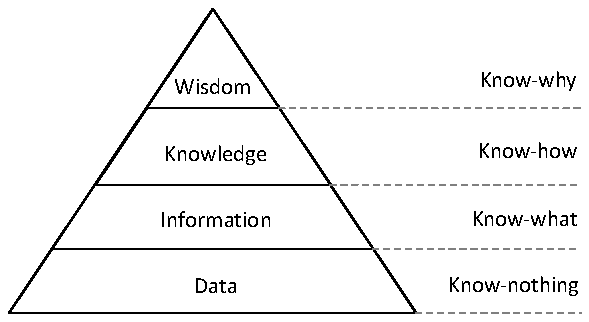
\includegraphics[scale=0.9]{img/example.pdf}
% 	\caption[Caption for the index]{Caption within the text \cite{Lauesen2002}.}
% 	\label{fig:example}
% \end{figure}

% Remember: 

% \begin{itemize}
%   \item Figures have to be referenced in the text using \texttt{\textbackslash
%   ref} and briefly explained. Do not worry if the image ends up on the following
%   page, probably there is no space to have it at the place where you inserted
%   it. 
%   \item Images should be vector images or saved with at least 600 dpi, so that
%   when printed they do not look blurry.
%   \item If the caption in the text and the index are the same, you can leave the
%   parameter for the caption for the index away, e.g., like
%   \texttt{\textbackslash caption\{Caption within the text.\}}
% \end{itemize}

% \textbf{Do not} use:

% \begin{tight_enumerate}
%   \item \texttt{\textbackslash begin\{figure\}[H!]} to force Latex to place a
%   figure where you want. Usually there is a good reason why a picture ends up
%   where it is positioned. Just refer to it with \texttt{\textbackslash ref} and
%   describe it. The reader is perfectly capable to find the image.
% \end{tight_enumerate}

% \section{Citations}
% You have to define reference material in a separate file called
% ``bibliography.bib''. Example of citations:
% \cite{Bass2012,Rubin2014,Dictionary1}. Have a look at \cite{rfc6824}.

% \section{Footnotes}
% Here is an example of a footnote\footnote{But do not use it too frequently :)}.
% Please use footnotes to provide the web site of any technology or product, e.g.,
% Microsoft Word\footnote{Microsoft Word,
% \url{http://office.microsoft.com/en-us/word}}, so that everyone knows what you
% are talking about.

% \section{Formulas}
% \LaTeX~is perfect for formulas: 
% \begin{equation}
% 	\label{equ:formula1}
% 	{\frac {d}{dx}}\arctan(\sin({x}^{2}))=-2\,{\frac {\cos({x}^{2})x}{-2+\left (\cos({x}^{2})\right )^{2}}}
% \end{equation}

% As you see in formula \ref{equ:formula1}, you can insert very nice formulas in
% your thesis too! Like figures, refer to the formula using \texttt{\textbackslash
% ref} and describe what the reader is seeing.

% \section{Tables}
% There are many ways to make a table, the table \ref{tab:tabExample} is a bit
% more complicated, but has many advantages, e.g., that you can have a table that
% breaks from one page to another.

% \begin{longtable}[c]{L{3cm}C{3cm}R{80pt}}
% \caption{Caption of the table within the text.} 
% \label{tab:tabExample} \\

% \toprule
% A & Header 2 & C \\
% \midrule
% \endfirsthead\longtableheader

% \toprule
% A & Header 2 & C \\
% \midrule
% \endhead\longtablefooter

% Left aligned & Center aligned & Right aligned \\
% Left aligned & Center aligned & Right aligned \\
% Left aligned & Center aligned & Right aligned \\
% Left aligned & Center aligned & Right aligned \\

% \end{longtable}

% Like for pictures and formulas, refer to the table using \texttt{\textbackslash
% ref} and describe what the reader is seeing.

% \textbf{Do not} use:

% \begin{tight_enumerate}
%   \item Vertical lines in a table
%   \item Double lines in a table
% \end{tight_enumerate}

% \section{Code}
% If you want to include code examples, you should use the \texttt{lstlisting}
% environment, as in listing \ref{lst:listing1}. 

% \begin{lstlisting}[caption=A listing example,label=lst:listing1]
% public ArrayList getList() {	
% 	ArrayList l = new ArrayList();
% 	Connection c = null;
% 	try {
% 		c = DatabaseTools.getConnection();
% 		Statement p = c.createStatement();
% 		ResultSet r = p.executeQuery("SELECT id, \"name\", readonly FROM \"group\" ORDER BY \"name\"");
% 		while (r.next()) {
% 			HashMap h = new HashMap();
% 			h.put("id", r.getString(1));
% 			h.put("name", r.getString(2));
% 			h.put("readonly", new Boolean(r.getBoolean(3)));
% 			l.add(h);
% 		}
% 	} catch (Exception e) {
% 		e.printStackTrace();
% 	} finally {
% 		if (c != null) {
% 			try {
% 				c.close();
% 			} catch (Exception e) {
% 				e.printStackTrace();
% 			}
% 		}
% 	}
	
% 	return l;
% }
% \end{lstlisting}

% Using the line numbers it is also easier to reference to them within the text.

% \section{Landscape}

% Sometimes, you need to show a picture or a table that requires a lot of space.
% To avoid that the text in the picture or table becomes unreadable, you can
% insert it in landscape mode, like the text on the next page.

% \begin{landscape}
% Some text in landscape mode.
% \end{landscape}
 

\bibliographystyle{unsrt}                                 
\bibliography{bibliography}

\end{document}
